\chapter{Chứng minh}

Toán học là duy nhất ở chỗ nó đòi hỏi một sự chắc chắn vượt xa mọi nghi ngờ hay tranh luận. Một chứng minh toán học cho thấy một kết quả nào đó được suy ra chỉ bằng logic từ một tập hợp các giả thiết đã cho, và một khi kết quả đã được chứng minh, nó vững chắc như chính nền tảng của logic. Tất nhiên, toán học đạt được sự chắc chắn này bằng cách tự giới hạn mình trong một thế giới toán học nhân tạo, và việc áp dụng nó vào thế giới thực không mang cùng mức độ chắc chắn.

Trong thế giới toán học, các hệ quả được suy ra từ các giả thiết với sức mạnh của logic, và một chứng minh chỉ đơn giản là cách chỉ ra các hệ quả logic. Tất nhiên, việc các kết quả toán học được suy ra một cách logic không có nghĩa là chúng hiển nhiên theo nghĩa thông thường. Các chứng minh thuyết phục một khi được phát hiện, nhưng việc tìm ra chúng thường rất khó khăn. Chúng được viết bằng một ngôn ngữ và phong cách có thể khó hiểu đối với người mới bắt đầu. Thường thì một chứng minh được xây dựng dựa trên một chuỗi dài các định nghĩa và kết quả trước đó, và trong khi mỗi bước trên đường đi có thể ``hiển nhiên'', kết quả cuối cùng có thể gây ngạc nhiên và mạnh mẽ. Đây chính là điều làm cho việc tìm kiếm các chứng minh trở nên xứng đáng.

Trong chương này, chúng ta sẽ xem xét một số cách tiếp cận và kỹ thuật có thể được sử dụng để chứng minh các kết quả toán học, bao gồm hai kỹ thuật chứng minh quan trọng được gọi là chứng minh phản chứng và quy nạp toán học. Trên đường đi, chúng ta sẽ gặp một vài định nghĩa và ký hiệu mới. Hy vọng rằng bạn sẽ có được mức độ tự tin cao hơn để khám phá thế giới toán học một mình.

%%%%%%%%%%%%%%%%%%%%%%%%%%%%%%%%%%%%%%%%%%%%%%%%%%%%%
\section{Một chút bối cảnh lịch sử}
%%%%%%%%%%%%%%%%%%%%%%%%%%%%%%%%%%%%%%%%%%%%%%%%%%%%%

Thế giới toán học và thế giới thực không phải lúc nào cũng tách biệt nhau như vậy. Cho đến khoảng giữa thế kỷ mười chín, các phát biểu của toán học được coi là các phát biểu về thế giới. Một chứng minh đơn giản chỉ là một lập luận thuyết phục, chứ không phải một chuỗi được rèn từ logic tuyệt đối. Nó gần hơn với nghĩa gốc của từ ``proof'' (chứng minh) trong tiếng Anh, như một phép thử hay thử thách: bạn có thể đã nghe câu tục ngữ ``The proof of the pudding is in the eating'' (muốn biết bánh pudding có ngon không thì phải nếm thử). Vì vậy, chứng minh một điều gì đó là kiểm tra tính đúng đắn của nó bằng cách đưa nó vào thử thách của lập luận logic.

\begin{warningbox}
Trong tiếng Anh, một lỗi thường gặp xoay quanh sự khác biệt giữa ``proof'' (danh từ) và ``to prove'' (động từ). Bạn có thể \emph{prove} (chứng minh) một khẳng định nào đó bằng cách sử dụng một \emph{proof} (chứng minh). Nhưng về mặt ngữ pháp, bạn không thể ``proof'' một khẳng định bằng một ``prove''. Trong lịch sử, ở môn học Reasoning \& Logic, đây là một trong những lỗi chính tả/ngữ pháp phổ biến nhất trong các bài thi. Bằng cách đưa nó vào cuốn sách này, chúng tôi hy vọng rằng bạn sẽ biết rõ hơn từ bây giờ.
\end{warningbox}

Tiếng sấm đầu tiên báo hiệu rắc rối đến dưới hình thức \textbf{hình học phi Euclid}. Trong hai nghìn năm, hình học của nhà toán học Hy Lạp Euclid đã được chấp nhận, đơn giản, là hình học của thế giới. Vào giữa thế kỷ mười chín, người ta phát hiện rằng có các hệ thống hình học khác, ít nhất cũng hợp lệ và tự nhất quán như hệ thống của Euclid. Các nhà toán học có thể làm việc trong bất kỳ hệ thống nào trong số này, nhưng không phải tất cả đều có thể tuyên bố đang làm việc trong thế giới thực.

Gần cuối thế kỷ mười chín, một cú sốc khác đến dưới dạng các vết nứt trong chính nền tảng của toán học. Vào thời điểm đó, nhà toán học Gottlob Frege đang hoàn thành một cuốn sách về lý thuyết tập hợp đại diện cho công trình cả đời của ông. Trong lý thuyết tập hợp của Frege, một tập hợp có thể được định nghĩa bởi bất kỳ tính chất nào. Bạn có thể có, ví dụ, tập hợp gồm tất cả các tập hợp chứa ba đối tượng. Khi ông đang hoàn thành cuốn sách, Frege nhận được một bức thư từ một nhà toán học trẻ tên là Bertrand Russell mô tả điều đã trở thành \textbf{Nghịch lý Russell}. Russell chỉ ra rằng tập hợp của tất cả các tập hợp---tức là, tập hợp chứa mọi thực thể thỏa mãn tính chất là một tập hợp---không thể tồn tại một cách logic. Chúng ta sẽ xem lập luận của Russell trong chương tiếp theo. Frege chỉ có thể thêm một lời bạt trong cuốn sách của mình nói rằng nền tảng của công trình đã bị quét sạch.

\begin{infobox}
Cùng thời với Peirce (xem trang 42), Friedrich Ludwig Gottlob Frege (1848--1925) là một nhà triết học, nhà logic học và nhà toán học người Đức. Peirce và Frege dường như hầu như không biết đến công trình của nhau. Frege được nhiều người hiểu là cha đẻ của triết học phân tích, tập trung vào triết học ngôn ngữ và toán học. Giống như Peirce, công trình của ông phần lớn bị bỏ qua trong suốt cuộc đời, và được các nhà toán học sau này công nhận---bao gồm Russell.

Nguồn: \texttt{en.wikipedia.org/wiki/Gottlob\_Frege}.
\end{infobox}

Các nhà toán học đã phản ứng với những vấn đề này bằng cách loại bỏ các viện dẫn đến sự thật về thế giới thực ra khỏi chứng minh toán học. Toán học phải là thế giới riêng của nó, được xây dựng trên nền tảng an toàn riêng. Nền tảng sẽ là một tập cơ bản các giả thiết hay ``tiên đề'' mà từ đó mọi thứ khác sẽ được suy ra bằng logic. Chỉ cần chứng minh rằng bản thân các tiên đề là nhất quán về mặt logic và đầy đủ, và thế giới toán học sẽ được an toàn. Thật không may, ngay cả điều này cũng không được như vậy. Vào những năm 1930, Kurt Gödel đã chứng minh rằng không có tập hữu hạn nhất quán các tiên đề nào mô tả đầy đủ ngay cả góc nhỏ của thế giới toán học được gọi là số học. Gödel chứng minh rằng cho bất kỳ tập hữu hạn, nhất quán các tiên đề nào, đều có các phát biểu đúng về số học mà không suy ra một cách logic từ các tiên đề đó. Chúng ta sẽ quay lại với Gödel và những người cùng thời trong Chương 5.

Chúng ta còn lại với một thế giới toán học trong đó các chuỗi sắt của logic vẫn ràng buộc kết luận với giả thiết. Nhưng các giả thiết không còn bắt nguồn từ thế giới thực. Cũng không có lõi hữu hạn nào của các tiên đề mà phần còn lại của thế giới toán học có thể được xích vào. Trong thế giới này, các tiên đề được đặt lên như những biển chỉ đường trong khoảng trống, và sau đó các cấu trúc logic được xây dựng xung quanh chúng. Ví dụ, trong chương tiếp theo, thay vì nói về \emph{lý thuyết} tập hợp mô tả thế giới thực, chúng ta có \emph{một} lý thuyết tập hợp, dựa trên một tập tiên đề cho trước. Lý thuyết tập hợp đó nhất thiết là không đầy đủ, và nó có thể khác với các lý thuyết tập hợp khác dựa trên các tập tiên đề khác.

%%%%%%%%%%%%%%%%%%%%%%%%%%%%%%%%%%%%%%%%%%%%%%%%%%%%%
\section{Chứng minh toán học}
%%%%%%%%%%%%%%%%%%%%%%%%%%%%%%%%%%%%%%%%%%%%%%%%%%%%%

Có thể hiểu được, các nhà toán học rất cầu kỳ trong việc làm đúng các chứng minh của họ. Đó là cách họ xây dựng thế giới của mình. Sinh viên đôi khi phản đối rằng các nhà toán học quá kỹ tính trong việc chứng minh những điều ``hiển nhiên''. Nhưng thực tế là một điều gì đó hiển nhiên trong thế giới thực có giá trị rất ít trong thế giới được xây dựng của toán học. Quá nhiều điều hiển nhiên đã hóa ra hoàn toàn sai. (Thực ra, ngay cả những điều trong thế giới thực mà dường như ``hiển nhiên'' đúng cũng không nhất thiết đúng chút nào.)

\begin{notebox}
Ví dụ, hãy xem xét đại lượng $f(n) = n^2 + n + 41$. Khi $n = 0$, $f(n) = 41$ là số nguyên tố; khi $n = 1$, $f(n) = 43$ là số nguyên tố; khi $n = 2$, $f(n) = 47$ là số nguyên tố. Khi bạn đã tính $f(3), f(4), \ldots, f(10)$ và thấy rằng chúng đều là số nguyên tố, bạn có thể kết luận rằng ``hiển nhiên'' rằng $f(n)$ là số nguyên tố cho mọi $n \geq 0$. Nhưng thực tế không phải vậy! (Xem bài tập.)
\end{notebox}

Như chúng ta đã thấy ở Mục 2.5, một chứng minh hình thức bao gồm một chuỗi các phát biểu trong đó mỗi phát biểu hoặc là một giả thiết hoặc được suy ra theo một quy tắc logic từ các phát biểu trước đó. Các ví dụ trong phần đó đều làm việc với các mệnh đề tổng quát không xác định ($p$, $q$, v.v.). Bây giờ chúng ta hãy xem xét cách sử dụng cùng các kỹ thuật đó để chứng minh một mệnh đề cụ thể về thế giới toán học. Chúng ta sẽ chứng minh rằng với mọi số nguyên $n$, nếu $n$ chẵn thì $n^2$ chẵn. (Định nghĩa: một số nguyên $n$ là \emph{chẵn} khi và chỉ khi $n = 2k$ với số nguyên $k$ nào đó. Ví dụ, $2$ là chẵn vì $2 = 2 \cdot 1$; $66$ là chẵn vì $66 = 2 \cdot 33$; $0$ là chẵn vì $0 = 2 \cdot 0$.)

\begin{proof}
Đây là một mệnh đề có dạng $\forall n(P(n) \to Q(n))$ trong đó $P(n)$ là ``$n$ chẵn'' và $Q(n)$ là ``$n^2$ chẵn.'' Chúng ta cần chứng minh rằng $P(n) \to Q(n)$ đúng với mọi giá trị của $n$. Hoặc nói cách khác chúng ta có thể phát biểu nó là: $\forall n(E(n) \to E(n^2))$ trong đó $E(x)$ là ``$x$ chẵn''.

Theo ngôn ngữ của Mục 2.5, chúng ta cần chứng minh rằng với mọi $n$, $E(n)$ suy ra logic $E(n^2)$; hoặc, tương đương, rằng $E(n^2)$ có thể được suy diễn logic từ $E(n)$; hoặc, tương đương, rằng
\begin{center}
$n$ chẵn\\
$\therefore\ n^2$ chẵn
\end{center}
là một lập luận hợp lệ. Đây là một chứng minh hình thức rằng
\begin{center}
$n$ chẵn\\
$\therefore\ n^2$ chẵn
\end{center}
thực sự là một lập luận hợp lệ cho bất kỳ giá trị nào của $n$:

Cho $n$ là một số nguyên tùy ý.
\begin{enumerate}
\item $n$ chẵn \hfill tiền đề
\item nếu $n$ chẵn, thì $n = 2k$ với số nguyên $k$ nào đó \hfill định nghĩa của chẵn
\item $n = 2k$ với số nguyên $k$ nào đó \hfill từ 1, 2 (\emph{modus ponens})
\item nếu $n = 2k$ với số nguyên $k$ nào đó, thì $n^2 = 4k^2$ với số nguyên $k$ đó \hfill đại số cơ bản
\item $n^2 = 4k^2$ với số nguyên $k$ nào đó \hfill từ 3, 4 (\emph{modus ponens})
\item nếu $n^2 = 4k^2$ với số nguyên $k$ nào đó, thì $n^2 = 2(2k^2)$ với $k$ đó \hfill đại số cơ bản
\item $n^2 = 2(2k^2)$ với số nguyên $k$ nào đó \hfill từ 5, 6 (\emph{modus ponens})
\item nếu $n^2 = 2(2k^2)$ với số nguyên $k$ nào đó, thì $n^2 = 2k'$ với số nguyên $k'$ nào đó \hfill tính chất cơ bản của số nguyên
\item $n^2 = 2k'$ với số nguyên $k'$ nào đó \hfill từ 7, 8 (\emph{modus ponens})
\item nếu $n^2 = 2k'$ với số nguyên $k'$ nào đó, thì $n^2$ chẵn \hfill định nghĩa của chẵn
\item $n^2$ chẵn \hfill từ 9, 10 (\emph{modus ponens})
\end{enumerate}

(``Tính chất cơ bản của số nguyên'' được đề cập ở trên là tích của các số nguyên lại là số nguyên.) Vì $n$ có thể được thay bởi bất kỳ số nguyên nào trong suốt lập luận này, chúng ta đã chứng minh rằng phát biểu ``nếu $n$ chẵn thì $n^2$ chẵn'' đúng với mọi số nguyên $n$. (Bạn có thể lo lắng rằng lập luận chỉ hợp lệ cho $n$ chẵn; xem phần nói về khả năng bóng đá của Feyenoord ở trang 54, hoặc nhắc mình rằng $P(n) \to Q(n)$ tự động đúng nếu $P(n)$ sai.)
\end{proof}

Các chứng minh toán học hiếm khi được trình bày với mức độ chi tiết và hình thức hóa như vậy. Một chứng minh ít hình thức hơn một chút cho mệnh đề của chúng ta có thể bỏ qua các kéo theo tường minh và các trường hợp \emph{modus ponens} và xuất hiện như sau:

\begin{proof}
Cho $n$ là một số nguyên tùy ý.
\begin{enumerate}
\item $n$ chẵn \hfill tiền đề
\item $n = 2k$ với số nguyên $k$ nào đó \hfill định nghĩa của chẵn
\item $n^2 = 4k^2$ với số nguyên $k$ đó \hfill đại số cơ bản
\item $n^2 = 2(2k^2)$ với $k$ đó \hfill đại số cơ bản
\item $n^2 = 2k'$ với số nguyên $k'$ nào đó \hfill thay $k' = 2k^2$
\item $n^2$ chẵn \hfill định nghĩa của chẵn
\end{enumerate}
Vì $n$ là số nguyên tùy ý, phát biểu đúng với mọi số nguyên.
\end{proof}

Một chứng minh điển hình hơn sẽ lấy lập luận ở trên và trình bày nó dưới dạng văn xuôi thay vì dạng danh sách:

\begin{proof}
Cho $n$ là một số nguyên tùy ý và giả sử $n$ chẵn. Khi đó $n = 2k$ với số nguyên $k$ nào đó theo định nghĩa của chẵn, và $n^2 = 4k^2 = 2(2k^2)$. Vì tích của các số nguyên là số nguyên, ta có $n^2 = 2k'$ với số nguyên $k'$ nào đó. Do đó $n^2$ chẵn. Vì $n$ là số nguyên tùy ý, phát biểu đúng với mọi số nguyên.
\end{proof}

Thông thường, trong một chứng minh ``hình thức'', chính loại thảo luận (tương đối) phi hình thức này được đưa ra, với đủ chi tiết để thuyết phục người đọc rằng một chứng minh hình thức đầy đủ có thể được xây dựng. Tất nhiên, bao nhiêu chi tiết người đọc có thể được kỳ vọng tự điền vào phụ thuộc vào người đọc, và đọc chứng minh là một kỹ năng phải được phát triển và thực hành.

\begin{warningbox}
Trong môn học Reasoning \& Logic, bạn đang học cách viết các chứng minh hình thức đúng, và là một phần trong đó chúng tôi cũng cần đánh giá thành tích của bạn. Để thực hiện điều này, chúng tôi yêu cầu bạn viết chứng minh tương tự như ví dụ thứ hai ở trên (dạng danh sách thay vì dạng văn xuôi) vì điều này cho thấy rõ ràng hơn rằng bạn nhận thức được các hình thức cần thiết trong một chứng minh.
\end{warningbox}

Viết một chứng minh còn khó hơn đọc một chứng minh. Mọi chứng minh đều liên quan đến một hành động sáng tạo khám phá, trong đó một chuỗi logic dẫn từ giả thiết đến kết luận được phát hiện. Nó cũng liên quan đến một hành động sáng tạo biểu đạt, trong đó logic đó được trình bày một cách rõ ràng và thuyết phục. Không có thuật toán nào để tạo ra các chứng minh đúng, mạch lạc. Tuy nhiên, có một số hướng dẫn chung để khám phá và viết chứng minh. Hãy xem xét một số trong đó tiếp theo.

\subsection{Cách viết một chứng minh}

Một trong những lời khuyên quan trọng nhất cần ghi nhớ là: ``Sử dụng định nghĩa''. Trong thế giới toán học, các thuật ngữ có nghĩa chính xác như chúng được định nghĩa và không gì hơn. Các định nghĩa cho phép tóm tắt các ý tưởng rất phức tạp thành các thuật ngữ đơn lẻ. Khi bạn đang cố chứng minh các điều về những thuật ngữ đó, bạn thường cần ``mở ra'' các định nghĩa. Trong ví dụ của chúng ta ở trên, chúng ta đã sử dụng định nghĩa của chẵn để viết $n = 2k$, và sau đó chúng ta làm việc với phương trình đó. Khi bạn đang cố chứng minh điều gì đó về quan hệ tương đương ở Chương 4, bạn có thể khá chắc chắn rằng bạn sẽ cần sử dụng thực tế là các quan hệ tương đương, theo định nghĩa, có tính đối xứng, phản xạ và bắc cầu. (Và tất nhiên, bạn sẽ cần biết thuật ngữ ``quan hệ'' được định nghĩa như thế nào ngay từ đầu! Chúng tôi muốn nói điều gì đó khác hoàn toàn so với ý tưởng rằng ``quan hệ'' là điều gì đó giống như cô chú của bạn.)

Thêm lời khuyên theo cùng hướng là kiểm tra xem bạn có đang sử dụng các giả thiết của định lý không. Một giả thiết được đặt ra trong một định lý được gọi là một \textbf{giả thuyết}. Các giả thuyết của định lý phát biểu các điều kiện mà tính đúng đắn của chúng sẽ đảm bảo kết luận của định lý. Chứng minh định lý có nghĩa là giả sử các giả thuyết đúng, và chỉ ra, dưới giả thiết đó, rằng kết luận phải đúng. Rất có khả năng (mặc dù không đảm bảo) rằng bạn sẽ cần sử dụng các giả thuyết một cách tường minh tại một điểm nào đó trong chứng minh, như chúng ta đã làm trong ví dụ trên.\footnote{Tất nhiên, nếu bạn tự khám phá các định lý mới, bạn không được cho trước các giả thuyết và kết luận từ đầu, điều này làm mọi thứ khó hơn nhiều---và thú vị hơn.} Ngoài ra, bạn nên nhớ rằng bất kỳ kết quả nào đã được chứng minh đều có thể sử dụng trong chứng minh của bạn.

Một chứng minh là một lập luận logic, dựa trên các quy tắc của logic. Vì thực sự không có quá nhiều quy tắc cơ bản của logic, các mẫu giống nhau liên tục xuất hiện. Hãy xem xét một số mẫu.

Mẫu phổ biến nhất xuất hiện trong nỗ lực chứng minh rằng điều gì đó đúng ``cho tất cả'' hay ``cho mọi'' hay ``cho bất kỳ'' thực thể nào trong một phạm trù cho trước. Theo thuật ngữ logic, phát biểu bạn đang cố chứng minh có dạng $\forall x\, P(x)$. Trong trường hợp này, cách có khả năng nhất để bắt đầu chứng minh là nói điều gì đó như: ``Cho $x$ là một thực thể tùy ý trong miền xét. Chúng ta muốn chứng minh rằng $P(x)$.'' Chúng ta gọi đây là \textbf{chứng minh bằng tổng quát hóa}. Trong phần còn lại của chứng minh, $x$ chỉ một thực thể không xác định nhưng xác định trong miền xét. Vì $x$ là tùy ý, chứng minh $P(x)$ tương đương với chứng minh $\forall x\, P(x)$. Bạn chỉ cần cẩn thận rằng bạn không sử dụng bất kỳ tính chất nào của $x$ ngoài những gì bạn đã giả thiết. Ví dụ, trong chứng minh ở trên, chúng ta không thể đặt bất kỳ giả thiết nào về số nguyên $n$ ngoài việc nó chẵn; nếu chúng ta ví dụ cũng giả sử $x = 6$ hoặc rằng $x$ chia hết cho $3$, thì chứng minh sẽ không đúng, hoặc ít nhất là không đầy đủ.

Đôi khi, bạn phải chứng minh rằng tồn tại một thực thể thỏa mãn các tính chất nhất định. Chứng minh như vậy được gọi là \textbf{chứng minh sự tồn tại}. Trong trường hợp này, bạn đang cố chứng minh một phát biểu có dạng $\exists x\, P(x)$. Cách để làm điều này là tìm một ví dụ, tức là tìm một thực thể cụ thể $a$ sao cho $P(a)$ đúng. Một cách để chứng minh phát biểu ``Có một số nguyên tố chẵn'' là tìm một số cụ thể thỏa mãn mô tả này. Cùng một phát biểu cũng có thể được diễn đạt ``Không phải mọi số nguyên tố đều lẻ.'' Phát biểu này có dạng $\neg(\forall x\, P(x))$, tương đương với phát biểu $\exists x(\neg P(x))$. Một ví dụ chứng minh phát biểu $\exists x(\neg P(x))$ cũng chứng minh $\neg(\forall x\, P(x))$. Ví dụ như vậy được gọi là một \textbf{phản ví dụ} cho phát biểu $\forall x\, P(x)$: Một phản ví dụ chứng minh rằng phát biểu $\forall x\, P(x)$ là sai. Số $2$ là một phản ví dụ cho phát biểu ``Mọi số nguyên tố đều lẻ.'' Thực tế, $2$ là phản ví dụ duy nhất cho phát biểu này; ngược lại, nhiều phát biểu có nhiều phản ví dụ.

Lưu ý rằng bây giờ chúng ta đã thảo luận cách chứng minh và bác bỏ các phát biểu lượng từ toàn thể, và cách chứng minh các phát biểu lượng từ tồn tại. Làm thế nào để bạn \emph{bác bỏ} $\exists x\, P(x)$? Nhớ rằng $\neg \exists x\, P(x)$ tương đương logic với $\forall x(\neg P(x))$, nên để bác bỏ $\exists x\, P(x)$ bạn cần chứng minh $\forall x(\neg P(x))$.

Nhiều phát biểu, giống như trong ví dụ của chúng ta ở trên, có dạng logic của một kéo theo, $p \to q$. (Chính xác hơn, chúng có dạng ``$\forall x(P(x) \to Q(x))$'', nhưng như đã thảo luận ở trên, chiến lược để chứng minh phát biểu như vậy là chứng minh $P(x) \to Q(x)$ cho một phần tử tùy ý $x$ của miền xét.) Phát biểu có thể là ``Với mọi số tự nhiên $n$, nếu $n$ chẵn thì $n^2$ chẵn,'' hoặc ``Với mọi xâu $x$, nếu $x$ thuộc ngôn ngữ $L$ thì $x$ được sinh bởi văn phạm $G$,''\footnote{Bạn sẽ học về điều này trong môn \emph{Automata, Computability and Complexity} ở năm thứ hai.} hoặc ``Với mọi phần tử $s$, nếu $s \in A$ thì $s \in B$.'' Đôi khi kéo theo là ngầm định chứ không tường minh: ví dụ, ``Tổng của hai số hữu tỷ là hữu tỷ'' thực sự là viết tắt cho ``Với mọi số $x$ và $y$, nếu $x$ và $y$ hữu tỷ thì $x + y$ hữu tỷ.'' Chứng minh của phát biểu như vậy thường bắt đầu bằng: ``Giả sử rằng $p$. Chúng ta muốn chứng minh rằng $q$.'' Trong phần còn lại của chứng minh, $p$ được coi là một giả thiết đã biết đúng. Như đã thảo luận ở trên, lập luận logic đằng sau điều này là bạn về cơ bản đang chứng minh rằng
\begin{center}
$p$\\
$\therefore\ q$
\end{center}
là một lập luận hợp lệ. Một cách khác để nghĩ về nó là nhớ rằng $p \to q$ tự động đúng trong trường hợp $p$ sai, nên không cần xử lý trường hợp đó tường minh. Trong trường hợp còn lại, khi $p$ đúng, chúng ta có thể chứng minh $p \to q$ đúng bằng cách chỉ ra rằng tính đúng của $q$ theo sau từ tính đúng của $p$. Vì vậy hãy nhớ rằng khi chứng minh một kéo theo bạn nên \emph{giả sử tiền đề và chứng minh hậu quả} (bạn có thể xem lại nghĩa của các từ đó ở trang 12).

Một phát biểu có dạng $p \wedge q$ có thể được chứng minh bằng cách chứng minh $p$ và $q$ riêng biệt. Một phát biểu có dạng $p \vee q$ có thể được chứng minh bằng cách chứng minh phát biểu tương đương logic $(\neg p) \to q$: để chứng minh $p \vee q$, bạn có thể giả sử $p$ sai và chứng minh, dưới giả thiết đó, rằng $q$ đúng. Ví dụ, phát biểu ``Mọi số nguyên là chẵn hoặc lẻ'' tương đương với phát biểu ``Mọi số nguyên không chẵn thì lẻ''.

Vì $p \leftrightarrow q$ tương đương với $(p \to q) \wedge (q \to p)$, một phát biểu có dạng $p \leftrightarrow q$ thường được chứng minh bằng cách đưa ra hai chứng minh, một cho $p \to q$ và một cho $q \to p$. Trong tiếng Anh, $p \leftrightarrow q$ có thể được phát biểu dưới nhiều dạng như ``$p$ khi và chỉ khi $q$'' (``$p$ if and only if $q$''), ``nếu $p$ thì $q$ và ngược lại,'' và ``$p$ là điều kiện cần và đủ cho $q$''. Cụm từ ``khi và chỉ khi'' (``if and only if'') rất phổ biến trong toán học nên nó thường được viết tắt là \emph{iff}.

Bạn cũng nên nhớ rằng bạn có thể chứng minh $p \to q$ bằng cách trình bày một chuỗi các kéo theo hợp lệ $p \to r \to s \to \cdots \to q$. Tương tự, $p \leftrightarrow q$ có thể được chứng minh bằng một chuỗi các tương đương khi và chỉ khi hợp lệ $p \leftrightarrow r \leftrightarrow s \leftrightarrow \cdots \leftrightarrow q$.

\subsection{Một số thuật ngữ}

Trước khi chúng ta xem xét một số chứng minh mẫu, đây là một số thuật ngữ mà chúng ta sẽ sử dụng trong suốt các chứng minh mẫu và phần còn lại của môn Reasoning \& Logic.
\begin{itemize}
\item \textbf{Số tự nhiên} (ký hiệu $\mathbb{N}$) là các số $0, 1, 2, \ldots$. Lưu ý rằng tổng và tích của các số tự nhiên là số tự nhiên.

\item \textbf{Số nguyên} (ký hiệu $\mathbb{Z}$) là các số $0, -1, 1, -2, 2, -3, 3, \ldots$. Lưu ý rằng tổng, tích và hiệu của các số nguyên là số nguyên.

\item \textbf{Số hữu tỷ} (ký hiệu $\mathbb{Q}$) là tất cả các số có thể viết dưới dạng $\dfrac{m}{n}$ trong đó $m$ và $n$ là số nguyên và $n \neq 0$. Vậy $\dfrac{1}{3}$ và $\dfrac{-65}{7}$ là các số hữu tỷ; ít hiển nhiên hơn, $6$ và $\dfrac{\sqrt{27}}{\sqrt{12}}$ cũng vậy vì $6 = \dfrac{6}{1}$ (hoặc, thực ra, $6 = \dfrac{-12}{-2}$), và $\dfrac{\sqrt{27}}{\sqrt{12}} = \sqrt{\dfrac{27}{12}} = \sqrt{\dfrac{9}{4}} = \dfrac{3}{2}$. Lưu ý hạn chế rằng số ở mẫu số không thể là $0$: $\dfrac{3}{0}$ hoàn toàn không phải là một số, hữu tỷ hay cách khác; nó là một đại lượng không xác định. Cũng lưu ý rằng tổng, tích, hiệu và thương của các số hữu tỷ là số hữu tỷ (với điều kiện bạn không chia cho $0$).

\item \textbf{Số thực} (ký hiệu $\mathbb{R}$) là các số có thể viết dưới dạng thập phân, có thể với vô hạn chữ số sau dấu thập phân. Lưu ý rằng tổng, tích, hiệu và thương của các số thực là số thực (với điều kiện bạn không chia cho $0$).

\item \textbf{Số vô tỷ} là các số thực không phải số hữu tỷ, tức là không thể viết dưới dạng tỷ số của hai số nguyên. Các số như vậy bao gồm $\sqrt{3}$ (mà chúng ta sẽ chứng minh không phải số hữu tỷ) và $\pi$ (nếu ai đã từng nói với bạn rằng $\pi = \dfrac{22}{7}$, hãy nhớ rằng $\dfrac{22}{7}$ chỉ là giá trị xấp xỉ của $\pi$). Sau này bạn sẽ học rằng chúng ta có thể mô tả tập hợp các số vô tỷ này là $\mathbb{R} - \mathbb{Q}$, tức là: nó bao gồm tất cả các số nằm trong $\mathbb{R}$ nhưng không nằm trong $\mathbb{Q}$.

\item Một số nguyên $n$ \textbf{chia hết} cho $m$ khi và chỉ khi $n = mk$ với số nguyên $k$ nào đó. Điều này cũng có thể được diễn đạt bằng cách nói rằng $m$ \emph{chia hết} $n$, với ký hiệu toán học $m \mid n$. Ví dụ, $2 \mid 8$, nhưng $8 \nmid 2$. $2 \mid n$ khi và chỉ khi $n = 2k$ với số nguyên $k$ nào đó; $n$ chia hết cho $3$ khi và chỉ khi $n = 3k$ với số nguyên $k$ nào đó, v.v. Lưu ý rằng nếu $2 \nmid n$ (tức là $n$ không chia hết cho $2$), thì $n$ phải lớn hơn bội của $2$ một đơn vị nên $n = 2k + 1$ với số nguyên $k$ nào đó. Tương tự, nếu $n$ không chia hết cho $3$ thì $n$ phải lớn hơn bội của $3$ một hoặc hai đơn vị, nên $n = 3k + 1$ hoặc $n = 3k + 2$ với số nguyên $k$ nào đó.

\item Một số nguyên là \textbf{chẵn} khi và chỉ khi nó chia hết cho $2$ và \textbf{lẻ} khi và chỉ khi không chia hết cho $2$.

\item Một số nguyên $n > 1$ là \textbf{số nguyên tố} nếu nó chia hết cho đúng hai số nguyên dương, cụ thể là $1$ và chính nó. Lưu ý rằng một số phải lớn hơn $1$ để có cơ hội được gọi là ``nguyên tố''. Đặc biệt, cả $0$ lẫn $1$ đều không phải số nguyên tố.
\end{itemize}

\subsection{Các ví dụ}

Bây giờ hãy xem một ví dụ khác về chứng minh. Chúng ta bắt đầu chứng minh rằng tổng của hai số hữu tỷ bất kỳ là hữu tỷ.

\begin{proof}
Chúng ta bắt đầu bằng cách giả sử $x$ và $y$ là các số hữu tỷ tùy ý. Đây là chứng minh hình thức rằng quy tắc suy luận
\begin{center}
$x$ hữu tỷ\\
$y$ hữu tỷ\\
$\therefore\ x + y$ hữu tỷ
\end{center}
là một quy tắc suy luận hợp lệ:
\begin{enumerate}
\item $x$ hữu tỷ \hfill tiền đề
\item nếu $x$ hữu tỷ, thì $x = \dfrac{a}{b}$ với các số nguyên $a$ và $b \neq 0$ \hfill định nghĩa số hữu tỷ
\item $x = \dfrac{a}{b}$ với các số nguyên $a$ và $b \neq 0$ \hfill từ 1, 2 (\emph{modus ponens})
\item $y$ hữu tỷ \hfill tiền đề
\item nếu $y$ hữu tỷ, thì $y = \dfrac{c}{d}$ với các số nguyên $c$ và $d \neq 0$ \hfill định nghĩa số hữu tỷ
\item $y = \dfrac{c}{d}$ với $c$ và $d \neq 0$ nào đó \hfill từ 4, 5 (\emph{modus ponens})
\item $x = \dfrac{a}{b}$ với $a$ và $b \neq 0$ nào đó và $y = \dfrac{c}{d}$ với $c$ và $d \neq 0$ nào đó \hfill từ 3, 6
\item nếu $x = \dfrac{a}{b}$ với $a$ và $b \neq 0$ nào đó và $y = \dfrac{c}{d}$ với $c$ và $d \neq 0$ thì $x + y = \dfrac{ad + bc}{bd}$ trong đó $a, b, c, d$ là số nguyên và $b, d \neq 0$ \hfill đại số cơ bản
\item $x + y = \dfrac{ad + bc}{bd}$ với $a, b, c, d$ nào đó trong đó $b, d \neq 0$ \hfill từ 7, 8 (\emph{modus ponens})
\item nếu $x + y = \dfrac{ad + bc}{bd}$ với $a, b, c, d$ nào đó trong đó $b, d \neq 0$ thì $x + y = \dfrac{m}{n}$ trong đó $m, n$ là số nguyên và $n \neq 0$ \hfill tính chất của số nguyên
\item $x + y = \dfrac{m}{n}$ trong đó $m$ và $n$ là số nguyên và $n \neq 0$ \hfill từ 9, 10 (\emph{modus ponens})
\item nếu $x + y = \dfrac{m}{n}$ trong đó $m$ và $n$ là số nguyên và $n \neq 0$ thì $x + y$ hữu tỷ \hfill định nghĩa số hữu tỷ
\item $x + y$ hữu tỷ \hfill từ 11, 12 (\emph{modus ponens})
\end{enumerate}

Vậy quy tắc suy luận ở trên là hợp lệ. Vì $x$ và $y$ là các số hữu tỷ tùy ý, chúng ta đã chứng minh rằng quy tắc hợp lệ cho mọi số hữu tỷ, và do đó tổng của hai số hữu tỷ bất kỳ là hữu tỷ.
\end{proof}

Một cách trình bày ít hình thức hơn mà chúng tôi mong đợi từ bạn trong môn học sẽ trông như sau:

\begin{proof}
Chứng minh bằng tổng quát hóa:
\begin{itemize}
\item Cho $x$ và $y$ là các số hữu tỷ tùy ý.
\item Theo định nghĩa số hữu tỷ, tồn tại các số nguyên $a, b \neq 0, c, d \neq 0$ sao cho $x = \dfrac{a}{b}$ và $y = \dfrac{c}{d}$.
\item Khi đó $x + y = \dfrac{ad + bc}{bd}$.
\item Chúng ta biết $ad + bc$ và $bd$ là số nguyên vì tổng và tích của các số nguyên là số nguyên, và chúng ta cũng biết $bd \neq 0$ vì cả $b$ lẫn $d$ đều khác $0$.
\item Vậy chúng ta đã viết $x + y$ dưới dạng tỷ số của hai số nguyên, với mẫu số khác không.
\item Do đó, theo định nghĩa số hữu tỷ, $x + y$ hữu tỷ.
\item Vì $x$ và $y$ là các số hữu tỷ tùy ý, tổng của hai số hữu tỷ bất kỳ là hữu tỷ.
\end{itemize}
\end{proof}

Và thêm một ví dụ nữa: chúng ta sẽ chứng minh rằng bất kỳ số có $4$ chữ số $d_1d_2d_3d_4$ nào đều chia hết cho $3$ khi và chỉ khi tổng của bốn chữ số chia hết cho $3$.

\begin{proof}
Phát biểu này có dạng $p \leftrightarrow q$; nhớ rằng $p \leftrightarrow q$ tương đương logic với $(p \to q) \wedge (q \to p)$. Vậy chúng ta cần chứng minh cho bất kỳ số $4$ chữ số $d_1d_2d_3d_4$ nào rằng (1) nếu $d_1d_2d_3d_4$ chia hết cho $3$ thì $d_1 + d_2 + d_3 + d_4$ chia hết cho $3$, và (2) nếu $d_1 + d_2 + d_3 + d_4$ chia hết cho $3$ thì $d_1d_2d_3d_4$ chia hết cho $3$. Cho $d_1d_2d_3d_4$ là một số $4$ chữ số tùy ý.

(1) Giả sử $d_1d_2d_3d_4$ chia hết cho $3$, tức là $d_1d_2d_3d_4 = 3k$ với số nguyên $k$ nào đó. Số $d_1d_2d_3d_4$ thực ra là $d_1 \times 1000 + d_2 \times 100 + d_3 \times 10 + d_4$, nên chúng ta có phương trình
\[d_1 \times 1000 + d_2 \times 100 + d_3 \times 10 + d_4 = 3k.\]
Vì $1000 = 999 + 1$, $100 = 99 + 1$, và $10 = 9 + 1$, phương trình này có thể viết lại
\[999d_1 + d_1 + 99d_2 + d_2 + 9d_3 + d_3 + d_4 = 3k.\]
Sắp xếp lại cho
\begin{align*}
d_1 + d_2 + d_3 + d_4 &= 3k - 999d_1 - 99d_2 - 9d_3 \\
&= 3k - 3(333d_1) - 3(33d_2) - 3(3d_3).
\end{align*}
Bây giờ chúng ta có thể phân tích $3$ từ vế phải để được
\[d_1 + d_2 + d_3 + d_4 = 3(k - 333d_1 - 33d_2 - d_3).\]
Vì $(k - 333d_1 - 33d_2 - d_3)$ là số nguyên, chúng ta đã chứng minh rằng $d_1 + d_2 + d_3 + d_4$ chia hết cho $3$.

(2) Giả sử $d_1 + d_2 + d_3 + d_4$ chia hết cho $3$. Xét số $d_1d_2d_3d_4$. Như đã nhận xét ở trên,
\[d_1d_2d_3d_4 = d_1 \times 1000 + d_2 \times 100 + d_3 \times 10 + d_4\]
nên
\begin{align*}
d_1d_2d_3d_4 &= 999d_1 + d_1 + 99d_2 + d_2 + 9d_3 + d_3 + d_4 \\
&= 999d_1 + 99d_2 + 9d_3 + (d_1 + d_2 + d_3 + d_4).
\end{align*}
Chúng ta đã giả sử $d_1 + d_2 + d_3 + d_4 = 3k$ với số nguyên $k$ nào đó, nên thay vào phương trình cuối cùng ta được
\[d_1d_2d_3d_4 = 999d_1 + 99d_2 + 9d_3 + 3k = 3(333d_1 + 33d_2 + 3d_3 + k).\]
Vì đại lượng trong ngoặc là số nguyên, chúng ta đã chứng minh rằng $d_1d_2d_3d_4$ chia hết cho $3$.

Trong (1) và (2) ở trên, số $d_1d_2d_3d_4$ là một số nguyên $4$ chữ số tùy ý, nên chúng ta đã chứng minh rằng cho mọi số nguyên $4$ chữ số, $d_1d_2d_3d_4$ chia hết cho $3$ khi và chỉ khi tổng của bốn chữ số chia hết cho $3$.
\end{proof}

Bây giờ giả sử chúng ta muốn chứng minh phát biểu ``Với mọi số nguyên $n$, $n^2$ chẵn khi và chỉ khi $n$ chẵn.'' Chúng ta đã chứng minh một nửa phát biểu này (``Với mọi số nguyên $n$, nếu $n$ chẵn thì $n^2$ chẵn''), nên tất cả những gì cần làm là chứng minh phát biểu ``Với mọi số nguyên $n$, nếu $n^2$ chẵn thì $n$ chẵn'' và chúng ta sẽ xong. Thật không may, điều này không đơn giản như nó có vẻ: giả sử chúng ta bắt đầu theo cách chuẩn và cho $n$ là số nguyên tùy ý và giả sử $n^2 = 2k$ với số nguyên $k$ nào đó. Khi đó chúng ta bị mắc kẹt! Lấy căn bậc hai cả hai vế sẽ cho ta $n$ ở vế trái nhưng sẽ để lại $\sqrt{2k}$ ở vế phải. Đại lượng này không có dạng $2k'$ với bất kỳ số nguyên $k'$ nào; nhân nó với $\dfrac{\sqrt{2}}{\sqrt{2}}$ sẽ cho $2\dfrac{\sqrt{k}}{\sqrt{2}}$ nhưng không có cách nào để chứng minh rằng $\dfrac{\sqrt{k}}{\sqrt{2}}$ là số nguyên. Vậy chúng ta đã đi vào ngõ cụt. Phải làm gì bây giờ?

Câu trả lời là chúng ta cần một kỹ thuật chứng minh khác. Các chứng minh mà chúng ta đã viết cho đến nay là những gì được gọi là \textbf{chứng minh trực tiếp}: để chứng minh $p \to q$ bạn giả sử $p$ đúng và chứng minh rằng tính đúng của $q$ theo sau. Đôi khi, khi chứng minh trực tiếp $p \to q$ thất bại, một \textbf{chứng minh gián tiếp} sẽ hiệu quả. Nhớ rằng \emph{đối ngẫu} của kéo theo $p \to q$ là kéo theo $\neg q \to \neg p$, và mệnh đề này tương đương logic với $p \to q$. Một chứng minh gián tiếp của $p \to q$, vì vậy, là chứng minh trực tiếp của đối ngẫu $\neg q \to \neg p$. Trong ví dụ hiện tại, thay vì chứng minh ``nếu $n^2$ chẵn thì $n$ chẵn'' trực tiếp, chúng ta có thể chứng minh đối ngẫu của nó ``nếu $n$ không chẵn (tức là $n$ lẻ) thì $n^2$ không chẵn (tức là $n^2$ lẻ)''. Chúng ta gọi phương pháp này là \textbf{chứng minh bằng đối ngẫu}. Chứng minh đối ngẫu này là một lập luận trực tiếp thông thường mà chúng tôi để lại cho bài tập.

Ngoài ra, đôi khi chúng ta cần \textbf{chứng minh bằng phân chia trường hợp}. Xem xét ví dụ rằng chúng ta muốn chứng minh $3 \mid (n^3 + 3n^2 + 2n)$ cho mọi số nguyên $n$. Điều chúng ta có thể làm là chia chứng minh thành ba trường hợp khác nhau dựa trên tính chia hết cho $3$. Nhớ từ định nghĩa tính chia hết rằng mọi số có thể viết dưới dạng $n = 3k$, $n = 3k + 1$, hoặc $n = 3k + 2$. Trong chứng minh bằng phân chia trường hợp, chúng ta chứng minh khẳng định đúng cho tất cả các trường hợp này và do đó chứng minh khẳng định đúng cho mọi số.

\subsection*{Bài tập}
\begin{exercise}
Tìm một số tự nhiên $n$ sao cho $n^2 + n + 41$ không phải số nguyên tố.
\end{exercise}

\begin{exercise}
Chứng minh rằng các mệnh đề $p \vee q$ và $(\neg p) \to q$ tương đương logic.
\end{exercise}

\begin{exercise}
Chứng minh rằng mệnh đề $(p \vee q) \to r$ tương đương với $(p \to r) \wedge (q \to r)$.
\end{exercise}

\begin{exercise}
Xác định mỗi phát biểu sau đây đúng hay sai. Nếu đúng, chứng minh nó. Nếu sai, cho phản ví dụ.
\begin{enumerate}[label=\alph*)]
\item Mọi số nguyên tố đều lẻ.
\item Mọi số nguyên tố lớn hơn $2$ đều lẻ.
\item Nếu $x$ và $y$ là các số nguyên với $x < y$, thì tồn tại số nguyên $z$ sao cho $x < z < y$.
\item Nếu $x$ và $y$ là các số thực với $x < y$, thì tồn tại số thực $z$ sao cho $x < z < y$.
\end{enumerate}
\end{exercise}

\begin{exercise}
Giả sử $r$, $s$ và $t$ là các số nguyên, sao cho $r$ chia hết $s$ và $s$ chia hết $t$. Chứng minh rằng $r$ chia hết $t$.
\end{exercise}

\begin{exercise}
Chứng minh rằng với mọi số nguyên $n$, nếu $n$ lẻ thì $n^2$ lẻ.
\end{exercise}

\begin{exercise}
Chứng minh rằng một số nguyên $n$ chia hết cho $3$ khi và chỉ khi $n^2$ chia hết cho $3$. (Gợi ý: đưa ra chứng minh gián tiếp cho ``nếu $n^2$ chia hết cho $3$ thì $n$ chia hết cho $3$.'')
\end{exercise}

\begin{exercise}
Chứng minh hoặc bác bỏ mỗi phát biểu sau. Nhớ rằng để bác bỏ một phát biểu chúng ta luôn cần một phản ví dụ!
\begin{enumerate}[label=\alph*)]
\item Tích của hai số nguyên chẵn là chẵn.
\item Tích của hai số nguyên là chẵn chỉ khi cả hai số nguyên đều chẵn.
\item Tích của hai số hữu tỷ là hữu tỷ.
\item Tích của hai số vô tỷ là vô tỷ.
\item Với mọi số nguyên $n$, nếu $n$ chia hết cho $4$ thì $n^2$ chia hết cho $4$.
\item Với mọi số nguyên $n$, nếu $n^2$ chia hết cho $4$ thì $n$ chia hết cho $4$.
\end{enumerate}
\end{exercise}

%%%%%%%%%%%%%%%%%%%%%%%%%%%%%%%%%%%%%%%%%%%%%%%%%%%%%
\section{Chứng minh phản chứng}
%%%%%%%%%%%%%%%%%%%%%%%%%%%%%%%%%%%%%%%%%%%%%%%%%%%%%

Giả sử rằng chúng ta bắt đầu với một tập hợp giả thiết nào đó và áp dụng các quy tắc logic để suy ra một chuỗi các phát biểu có thể được chứng minh từ những giả thiết đó, và giả sử rằng chúng ta suy ra một phát biểu mà chúng ta biết là sai. Khi các quy tắc logic được áp dụng cho các phát biểu đúng, các phát biểu được suy ra cũng sẽ đúng. Nếu chúng ta suy ra một phát biểu sai bằng cách áp dụng các quy tắc logic cho một tập giả thiết, thì ít nhất một trong các giả thiết phải sai. Quan sát này dẫn đến một kỹ thuật chứng minh mạnh mẽ, được gọi là \textbf{chứng minh phản chứng}.

Giả sử bạn muốn chứng minh một mệnh đề $p$ nào đó. Để áp dụng chứng minh phản chứng, giả sử $\neg p$ đúng, và áp dụng các quy tắc logic để suy ra các kết luận dựa trên giả thiết này. Nếu có thể suy ra một phát biểu được biết là sai, suy ra rằng giả thiết $\neg p$ phải sai. (Tất nhiên, nếu suy dẫn dựa trên nhiều giả thiết, thì bạn chỉ biết rằng ít nhất một trong các giả thiết phải sai.) Thực tế là $\neg p$ sai chứng minh rằng $p$ đúng. Về bản chất, bạn đang lập luận rằng $p$ phải đúng, bởi vì nếu không, thì một phát biểu nào đó được biết là sai có thể được chứng minh là đúng. Thông thường, phát biểu sai được suy ra trong chứng minh phản chứng có dạng $q \wedge \neg q$. Phát biểu này là mâu thuẫn theo nghĩa nó sai bất kể giá trị của $q$. Lưu ý rằng việc suy ra mâu thuẫn $q \wedge \neg q$ giống như việc chứng minh rằng hai phát biểu $q$ và $\neg q$ đều theo sau từ giả thiết $\neg p$.

Như một ví dụ đầu tiên về chứng minh phản chứng, xét định lý sau:

\begin{theorem}
Số $\sqrt{3}$ là vô tỷ.
\end{theorem}

\begin{proof}
Chứng minh phản chứng:
\begin{itemize}
\item Giả sử để dẫn đến mâu thuẫn rằng $\sqrt{3}$ là hữu tỷ.
\item Khi đó $\sqrt{3}$ có thể viết dưới dạng tỷ số của hai số nguyên, $\sqrt{3} = \dfrac{m'}{n'}$ với các số nguyên $m'$ và $n'$ nào đó.
\item Hơn nữa, phân số $\dfrac{m'}{n'}$ có thể được rút gọn về dạng tối giản bằng cách triệt tiêu tất cả các thừa số chung của $m'$ và $n'$. Vậy $\sqrt{3} = \dfrac{m}{n}$ với các số nguyên $m$ và $n$ không có thừa số chung.
\item Bình phương cả hai vế của phương trình này cho $3 = \dfrac{m^2}{n^2}$ và sắp xếp lại cho $3n^2 = m^2$.
\item Từ phương trình này ta thấy $m^2$ chia hết cho $3$; bạn đã chứng minh ở phần trước (Bài tập 6) rằng $m^2$ chia hết cho $3$ khi và chỉ khi $m$ chia hết cho $3$. Do đó $m$ chia hết cho $3$ và ta có thể viết $m = 3k$ với số nguyên $k$ nào đó.
\item Thay $m = 3k$ vào phương trình cuối ở trên cho $3n^2 = (3k)^2$ hay $3n^2 = 9k^2$, từ đó $n^2 = 3k^2$. Từ đây ta thấy $n^2$ chia hết cho $3$, và lại ta biết rằng điều này suy ra $n$ chia hết cho $3$.
\item Nhưng bây giờ ta có (i) $m$ và $n$ không có thừa số chung, và (ii) $m$ và $n$ có thừa số chung, cụ thể là $3$. Không thể cả hai điều này đều đúng, nhưng lập luận của ta đã đúng về mặt logic.
\item Do đó giả thiết ban đầu, rằng $\sqrt{3}$ hữu tỷ, phải sai.
\item Do đó $\sqrt{3}$ phải là vô tỷ.
\end{itemize}
\end{proof}

Một trong những chứng minh toán học lâu đời nhất, quay ngược lại tận Euclid, là một chứng minh phản chứng. Nhớ rằng số nguyên tố là một số nguyên $n$, lớn hơn $1$, sao cho chỉ có các số nguyên dương chia hết $n$ là $1$ và $n$. Chúng ta sẽ chứng minh rằng có vô hạn số nguyên tố. Trước khi đến định lý, chúng ta cần một bổ đề. (Bổ đề là một định lý được đưa ra chỉ vì nó cần thiết trong chứng minh của định lý khác. Các bổ đề giúp tổ chức chứng minh của một định lý lớn thành các phần có thể quản lý được.)

\begin{lemma}
Nếu $N$ là một số nguyên và $N > 1$, thì tồn tại một số nguyên tố chia hết $N$.
\end{lemma}

\begin{proof}
Cho $D$ là số nguyên nhỏ nhất lớn hơn $1$ và chia hết $N$. ($D$ tồn tại vì có ít nhất một số, cụ thể là chính $N$, lớn hơn $1$ và chia hết $N$. Chúng ta sử dụng thực tế rằng mọi tập con không rỗng của $\mathbb{N}$ có phần tử nhỏ nhất.) Chúng ta khẳng định rằng $D$ là số nguyên tố, sao cho $D$ là một số nguyên tố chia hết $N$.

Giả sử $D$ không phải số nguyên tố. Chúng ta chứng minh rằng giả thiết này dẫn đến mâu thuẫn. Vì $D$ không nguyên tố, thì theo định nghĩa, tồn tại số $k$ nằm giữa $2$ và $D - 1$, bao gồm cả hai đầu, sao cho $k$ chia hết $D$. Nhưng vì $D$ chia hết $N$, chúng ta cũng có $k$ chia hết $N$ (theo bài tập 5 ở phần trước). Tức là, $k$ là một số nguyên lớn hơn một và chia hết $N$. Nhưng vì $k$ nhỏ hơn $D$, điều này mâu thuẫn với thực tế rằng $D$ là số nhỏ nhất như vậy. Mâu thuẫn này chứng minh rằng $D$ là số nguyên tố.
\end{proof}

\begin{theorem}
Có vô hạn số nguyên tố.
\end{theorem}

\begin{proof}
Giả sử rằng chỉ có hữu hạn số nguyên tố. Chúng ta sẽ chứng minh rằng giả thiết này dẫn đến mâu thuẫn.

Cho $p_1, p_2, \ldots, p_n$ là danh sách đầy đủ của tất cả các số nguyên tố (tồn tại dưới giả thiết rằng chỉ có hữu hạn số nguyên tố). Xét số $N$ có được bằng cách nhân tất cả các số nguyên tố và cộng thêm một. Tức là,
\[N = (p_1 \cdot p_2 \cdot p_3 \cdots p_n) + 1.\]
Bây giờ, vì $N$ lớn hơn bất kỳ số nguyên tố $p_i$ nào, và vì $p_1, p_2, \ldots, p_n$ là danh sách đầy đủ các số nguyên tố, chúng ta biết rằng $N$ không thể là số nguyên tố. Theo bổ đề, tồn tại một số nguyên tố $p$ chia hết $N$. Bây giờ, $p$ phải là một trong các số $p_1, p_2, \ldots, p_n$. Nhưng thực tế, không có số nào trong số này chia hết $N$, vì chia $N$ cho bất kỳ $p_i$ nào đều dư $1$. Mâu thuẫn này chứng minh rằng giả thiết chỉ có hữu hạn số nguyên tố là sai.
\end{proof}

Chứng minh này thể hiện sức mạnh của chứng minh phản chứng. Thực tế được chứng minh ở đây hoàn toàn không hiển nhiên, thế nhưng nó có thể được chứng minh chỉ trong vài đoạn văn.

\subsection*{Bài tập}
\begin{exercise}
Giả sử $a_1, a_2, \ldots, a_{10}$ là các số thực, và giả sử $a_1 + a_2 + \cdots + a_{10} > 100$. Sử dụng chứng minh phản chứng để kết luận rằng ít nhất một trong các số $a_i$ phải lớn hơn $10$.
\end{exercise}

\begin{exercise}
Chứng minh rằng mỗi phát biểu sau đây đúng. Trong mỗi trường hợp, sử dụng chứng minh phản chứng. Nhớ rằng phủ định của $p \to q$ là $p \wedge \neg q$.
\begin{enumerate}[label=\alph*)]
\item Cho $n$ là một số nguyên. Nếu $n^2$ là số nguyên chẵn, thì $n$ là số nguyên chẵn.
\item $\sqrt{2}$ là vô tỷ.
\item Nếu $r$ là số hữu tỷ và $x$ là số vô tỷ, thì $r + x$ là số vô tỷ. (Tức là, tổng của một số hữu tỷ và một số vô tỷ là vô tỷ.)
\item Nếu $r$ là số hữu tỷ khác không và $x$ là số vô tỷ, thì $rx$ là số vô tỷ.
\item Nếu $r$ và $r + x$ đều hữu tỷ, thì $x$ hữu tỷ.
\end{enumerate}
\end{exercise}

\begin{exercise}
\textbf{Nguyên lý chuồng bồ câu} là nhận xét hiển nhiên sau: Nếu bạn có $n$ con bồ câu trong $k$ chuồng và nếu $n > k$, thì có ít nhất một chuồng chứa nhiều hơn một con bồ câu. Mặc dù nhận xét này có vẻ hiển nhiên, nhưng chứng minh nó là ý tưởng tốt. Chứng minh nguyên lý chuồng bồ câu bằng chứng minh phản chứng.
\end{exercise}

%%%%%%%%%%%%%%%%%%%%%%%%%%%%%%%%%%%%%%%%%%%%%%%%%%%%%
\section{Quy nạp toán học}
%%%%%%%%%%%%%%%%%%%%%%%%%%%%%%%%%%%%%%%%%%%%%%%%%%%%%

Cấu trúc của các số tự nhiên---$0, 1, 2, 3$, và tiếp tục đến vô cùng---tạo nên một kỹ thuật chứng minh mạnh mẽ gọi là \textbf{quy nạp} hay \textbf{quy nạp toán học}. Mặc dù ý tưởng đằng sau quy nạp đơn giản, sinh viên thường gặp khó khăn với nó. Hãy dành thời gian và nghiên cứu tài liệu này kỹ lưỡng! Bạn sẽ có cơ hội thực hành trong các buổi lab sau khi chúng tôi thảo luận về quy nạp trong bài giảng.

Cho $P$ là một vị từ một ngôi có miền xét bao gồm các số tự nhiên. Giả sử rằng chúng ta có thể chứng minh $P(0)$ đúng. Giả sử rằng chúng ta cũng có thể chứng minh các phát biểu $P(0) \to P(1)$, $P(1) \to P(2)$, $P(2) \to P(3)$, v.v. Nguyên lý quy nạp toán học là quan sát rằng khi đó chúng ta có thể kết luận $P(n)$ đúng cho mọi số tự nhiên $n$. Điều này nên rõ ràng. Nó giống như một hàng domino, xếp hàng và sẵn sàng đổ, cái này sau cái kia. Vì $P(0)$ và $P(0) \to P(1)$ đúng, chúng ta có thể áp dụng quy tắc \emph{modus ponens} để kết luận $P(1)$ đúng. Sau đó, vì $P(1)$ và $P(1) \to P(2)$ đúng, chúng ta có thể kết luận bằng \emph{modus ponens} rằng $P(2)$ đúng. Từ $P(2)$ và $P(2) \to P(3)$, chúng ta kết luận $P(3)$ đúng. Cho bất kỳ $n$ nào trong tập $\mathbb{N}$, chúng ta có thể tiếp tục chuỗi suy diễn này $n$ bước để chứng minh $P(n)$ đúng.

Khi áp dụng quy nạp, chúng ta không thực sự chứng minh từng kéo theo $P(0) \to P(1)$, $P(1) \to P(2)$, v.v., riêng lẻ. Điều đó sẽ đòi hỏi lượng công việc vô hạn. Toàn bộ ý nghĩa của quy nạp là tránh mọi quá trình dài vô hạn. Thay vào đó, chúng ta chứng minh $\forall k(P(k) \to P(k+1))$ (trong đó miền xét cho vị từ $P$ là $\mathbb{N}$). Phát biểu $\forall k(P(k) \to P(k+1))$ tóm tắt tất cả vô hạn kéo theo trong một phát biểu duy nhất. Phát biểu chính thức, nguyên lý quy nạp toán học nói rằng nếu chúng ta có thể chứng minh phát biểu $P(0) \wedge \forall k(P(k) \to P(k+1))$, thì chúng ta có thể suy ra $\forall n\, P(n)$ (lại với $\mathbb{N}$ là miền xét).

\subsection{Cách viết chứng minh quy nạp}

Nên rõ ràng một cách trực giác rằng nguyên lý quy nạp là hợp lệ. Nó được suy ra từ thực tế rằng danh sách $0, 1, 2, 3, \ldots$, nếu kéo dài đủ, cuối cùng sẽ bao gồm bất kỳ số tự nhiên cho trước nào. Nếu chúng ta bắt đầu từ $P(0)$ và thực hiện đủ bước dạng $P(k) \to P(k+1)$, chúng ta có thể đạt $P(n)$ cho bất kỳ số tự nhiên $n$ cho trước nào. Tuy nhiên, bất cứ khi nào chúng ta xử lý vô hạn, chúng ta đang đùa giỡn với khả năng nghịch lý. Chúng ta sẽ chứng minh nguyên lý quy nạp một cách chặt chẽ trong chương tiếp theo (xem Định lý 4.3), nhưng hiện tại chúng ta chỉ phát biểu nó như một định lý:

\begin{theorem}
Cho $P$ là một vị từ một ngôi có miền xét bao gồm các số tự nhiên. Giả sử rằng $P(0) \wedge \big(\forall k \in \mathbb{N}\, (P(k) \to P(k+1))\big)$.\footnote{Chúng ta sẽ gặp ký hiệu $k \in \mathbb{N}$ này lại ở Chương 4. Hiện tại bạn chỉ cần nhớ rằng $k \in \mathbb{N}$ nghĩa là: $k$ là một số nguyên từ tập $\mathbb{N}$.} Khi đó $P(n)$ đúng cho mọi số tự nhiên $n$. (Tức là, phát biểu $\forall n\, P(n)$ đúng, trong đó miền xét cho $P$ là tập các số tự nhiên.)
\end{theorem}

Quy nạp toán học có thể được áp dụng trong nhiều tình huống: bạn có thể chứng minh các điều về xâu ký tự bằng cách quy nạp theo độ dài xâu, các điều về đồ thị bằng cách quy nạp theo số đỉnh, các điều về văn phạm bằng cách quy nạp theo số luật sinh, v.v. Chúng ta sẽ xem xét các ứng dụng của quy nạp trong phần còn lại của chương này, và xử lý một dạng gọi là quy nạp cấu trúc trong chương tiếp theo.

Mặc dù các chứng minh quy nạp có thể rất khác nhau, chúng đều tuân theo chỉ vài cấu trúc cơ bản. Một chứng minh dựa trên định lý trên luôn có hai phần. Đầu tiên, $P(0)$ được chứng minh. Đây được gọi là \textbf{trường hợp cơ sở} của quy nạp. Sau đó phát biểu $\forall k(P(k) \to P(k+1))$ được chứng minh. Phát biểu này có thể được chứng minh bằng cách cho $k$ là phần tử tùy ý của $\mathbb{N}$ và chứng minh $P(k) \to P(k+1)$. Điều này lần lượt có thể được chứng minh bằng cách giả sử $P(k)$ đúng và chứng minh rằng tính đúng của $P(k+1)$ theo sau từ giả thiết đó. Trường hợp này được gọi là \textbf{bước quy nạp}, và $P(k)$ được gọi là \textbf{giả thiết quy nạp} hay \textbf{giả thuyết quy nạp}. Lưu ý rằng trường hợp cơ sở quan trọng không kém bước quy nạp. Tự thân nó, tính đúng của phát biểu $\forall k(P(k) \to P(k+1))$ không nói gì về tính đúng của bất kỳ phát biểu $P(n)$ riêng lẻ nào. Chuỗi kéo theo $P(0) \to P(1)$, $P(1) \to P(2)$, \ldots, $P(n-1) \to P(n)$ không nói gì về $P(n)$ trừ khi chuỗi được neo ở đầu kia bởi tính đúng của $P(0)$.

\subsection{Các ví dụ}

Hãy xem xét một vài ví dụ.

\begin{theorem}
Số $2^{2n} - 1$ chia hết cho $3$ với mọi số tự nhiên $n$.
\end{theorem}

\begin{proof}
Ở đây, $P(n)$ là phát biểu rằng $2^{2n} - 1$ chia hết cho $3$.

\textbf{Trường hợp cơ sở:} Khi $n = 0$, $2^{2n} - 1 = 2^0 - 1 = 1 - 1 = 0$ và $0$ chia hết cho $3$ (vì $0 = 3 \cdot 0$). Do đó phát biểu đúng khi $n = 0$.

\textbf{Bước quy nạp:} Chúng ta muốn chứng minh rằng nếu phát biểu đúng cho $n = k$ (trong đó $k$ là số tự nhiên tùy ý), thì nó cũng đúng cho $n = k + 1$. Tức là, chúng ta phải chứng minh kéo theo $P(k) \to P(k+1)$. Vậy chúng ta giả sử $P(k)$, tức là chúng ta giả sử $2^{2k}$ chia hết cho $3$. Điều này nghĩa là $2^{2k} - 1 = 3m$ với số nguyên $m$ nào đó. Chúng ta muốn chứng minh $P(k+1)$, tức là $2^{2(k+1)} - 1$ cũng chia hết cho $3$:
\begin{align*}
2^{2(k+1)} - 1 &= 2^{2k+2} - 1 \\
&= 2^{2k} \cdot 2^2 - 1 && \text{tính chất của lũy thừa}\\
&= 4 \cdot 2^{2k} - 1 \\
&= 4 \cdot 2^{2k} - 4 + 4 - 1 \\
&= 4(2^{2k} - 1) + 3 && \text{đại số}\\
&= 4(3m) + 3 && \text{giả thiết quy nạp}\\
&= 3(4m + 1) && \text{đại số}
\end{align*}
và từ dòng cuối ta thấy $2^{2(k+1)} - 1$ thực sự chia hết cho $3$. (Bước thứ ba---trừ rồi cộng $4$---được thực hiện để cho phép chúng ta sử dụng giả thiết quy nạp.)

Tổng hợp lại, chúng ta đã chứng minh $P(0)$ đúng và rằng với mọi $k$, $P(k) \to P(k+1)$ đúng. Do đó, theo nguyên lý quy nạp, $P(n)$ đúng cho mọi $n$ trong $\mathbb{N}$, tức là $2^{2n} - 1$ chia hết cho $3$ với mọi $n$ trong $\mathbb{N}$.
\end{proof}

Nguyên lý quy nạp toán học cho một phương pháp chứng minh $P(n)$ cho mọi $n$ trong tập $\mathbb{N}$. Nên rõ ràng rằng nếu $M$ là bất kỳ số tự nhiên nào, một phương pháp tương tự có thể được sử dụng để chứng minh $P(n)$ đúng cho mọi số tự nhiên $n$ thỏa mãn $n \geq M$. Chỉ cần bắt đầu quy nạp với trường hợp cơ sở $n = M$ thay vì $n = 0$. Chúng tôi để chứng minh mở rộng này của nguyên lý quy nạp như bài tập. Chúng ta có thể sử dụng nguyên lý mở rộng này để chứng minh một kết quả đã được đề cập lần đầu ở Mục 2.1.

\begin{theorem}
Giả sử một mệnh đề hợp chứa đúng $n$ biến mệnh đề, trong đó $n \geq 1$. Khi đó có đúng $2^n$ cách khác nhau để gán giá trị chân lý cho $n$ biến.
\end{theorem}

\begin{proof}
Cho $P(n)$ là phát biểu ``Có đúng $2^n$ cách khác nhau để gán giá trị chân lý cho $n$ biến mệnh đề.'' Chúng ta sử dụng quy nạp để chứng minh $P(n)$ đúng cho mọi $n \geq 1$.

\textbf{Trường hợp cơ sở:} Đầu tiên, chúng ta chứng minh phát biểu $P(1)$. Nếu có đúng một biến, thì có đúng hai cách gán giá trị chân lý cho biến đó. Cụ thể, biến có thể đúng hoặc sai. Vì $2 = 2^1$, $P(1)$ đúng.

\textbf{Bước quy nạp:} Giả sử $P(k)$ đã biết đúng. Chúng ta muốn chứng minh rằng, dưới giả thiết này, $P(k+1)$ cũng đúng. Giả sử $p_1, p_2, \ldots, p_{k+1}$ là $k + 1$ biến mệnh đề. Vì chúng ta giả sử $P(k)$ đúng, chúng ta biết có $2^k$ cách gán giá trị chân lý cho $p_1, p_2, \ldots, p_k$. Nhưng mỗi phép gán giá trị chân lý cho $p_1, p_2, \ldots, p_k$ có thể được mở rộng thành danh sách đầy đủ $p_1, p_2, \ldots, p_k, p_{k+1}$ theo hai cách. Cụ thể, $p_{k+1}$ có thể được gán giá trị đúng hoặc sai. Suy ra có $2 \cdot 2^k$ cách gán giá trị chân lý cho $p_1, p_2, \ldots, p_{k+1}$. Vì $2 \cdot 2^k = 2^{k+1}$, điều này hoàn thành chứng minh.
\end{proof}

\subsection{Thêm ví dụ}

Tổng của một số lượng số hạng tùy ý được viết bằng ký hiệu $\sum$. (Ký hiệu này là chữ cái Hy Lạp sigma, tương đương với chữ cái La-tinh S và viết tắt cho ``sum'' (tổng).) Do đó, chúng ta có
\[\sum_{i=1}^{5} i^2 = 1^2 + 2^2 + 3^2 + 4^2 + 5^2\]
\[\sum_{k=3}^{7} a_k = a_3 + a_4 + a_5 + a_6 + a_7\]
\[\sum_{n=0}^{N} \frac{1}{n+1} = \frac{1}{0+1} + \frac{1}{1+1} + \frac{1}{2+1} + \cdots + \frac{1}{N+1}\]

Ký hiệu này cho tổng, sử dụng toán tử $\sum$, được gọi là \textbf{ký hiệu tổng}. Một ký hiệu tương tự cho tích sử dụng ký hiệu $\prod$. (Đây là chữ cái Hy Lạp pi, tương đương với chữ La-tinh P và viết tắt cho ``product'' (tích).) Ví dụ,
\[\prod_{k=2}^{5} (3k + 2) = (3 \cdot 2 + 2)(3 \cdot 3 + 2)(3 \cdot 4 + 2)(3 \cdot 5 + 2)\]
\[\prod_{i=1}^{n} \frac{1}{i} = \frac{1}{1} \cdot \frac{1}{2} \cdots \frac{1}{n}\]

Quy nạp có thể được sử dụng để chứng minh nhiều công thức sử dụng các ký hiệu này. Đây là hai ví dụ:

\begin{theorem}
$\displaystyle\sum_{i=1}^{n} i = \frac{n(n+1)}{2}$ với mọi số nguyên $n$ lớn hơn không.
\end{theorem}

Chúng ta sẽ chứng minh định lý này trên lớp. Bạn có thể tự làm không?

\begin{infobox}
Phép tổng ở Định lý 3.7 thường được gán cho nhà toán học và vật lý học Carl Friedrich Gauss (1777--1855). Gauss có ảnh hưởng đặc biệt lớn trong nhiều lĩnh vực; ông được gọi là ``nhà toán học vĩ đại nhất kể từ thời cổ đại''. Ví dụ, bạn có thể đã nghe về phân phối xác suất Gauss, hoặc có lẽ đơn vị Gauss cho từ thông (mặc dù ngày nay chúng ta thường dùng Tesla cho điều đó, với $1$ Tesla bằng $10^5$ Gauss). Sự xuất sắc của ông đã rõ ràng từ khi học tiểu học khi ông được cho là đã sử dụng ``tổng Gauss'' từ Định lý 3.7 để giải bài toán về nhà mà giáo viên đã giao cho cả lớp---khiến giáo viên vô cùng kinh ngạc. Bạn sẽ gặp lại phép tổng này trong môn \emph{Algorithms \& Data Structures} khi phân tích thời gian chạy của các thuật toán chứa vòng lặp.

Nguồn: \texttt{en.wikipedia.org/wiki/Carl\_Friedrich\_Gauss}.
\end{infobox}

\begin{theorem}
$\displaystyle\sum_{i=1}^{n} i \cdot 2^{i-1} = (n-1) \cdot 2^n + 1$ với mọi số tự nhiên $n > 0$.
\end{theorem}

\begin{proof}
Cho $P(n)$ là phát biểu $\displaystyle\sum_{i=1}^{n} i \cdot 2^{i-1} = (n-1) \cdot 2^n + 1$. Chúng ta sử dụng quy nạp để chứng minh $P(n)$ đúng cho mọi $n > 0$.

\textbf{Trường hợp cơ sở:} Xét trường hợp $n = 1$. $P(1)$ là phát biểu rằng $\displaystyle\sum_{i=1}^{1} i \cdot 2^{i-1} = (1-1) \cdot 2^1 + 1$. Vì mỗi vế của phương trình này bằng một, điều này đúng.

\textbf{Bước quy nạp:} Cho $k \geq 1$ tùy ý, và giả sử $P(k)$ đúng. Chúng ta muốn chứng minh $P(k+1)$ đúng. $P(k+1)$ là phát biểu $\displaystyle\sum_{i=1}^{k+1} i \cdot 2^{i-1} = ((k+1)-1) \cdot 2^{k+1} + 1$. Nhưng chúng ta có thể tính rằng
\begin{align*}
\sum_{i=1}^{k+1} i \cdot 2^{i-1} &= \left(\sum_{i=1}^{k} i \cdot 2^{i-1}\right) + (k+1) \cdot 2^{(k+1)-1} \\
&= \big((k-1) \cdot 2^k + 1\big) + (k+1) \cdot 2^k && \text{(giả thiết quy nạp)}\\
&= \big((k-1) + (k+1)\big) \cdot 2^k + 1 \\
&= (k \cdot 2) \cdot 2^k + 1 \\
&= k \cdot 2^{k+1} + 1
\end{align*}
đó là điều chúng ta muốn chứng minh. Điều này hoàn thành quy nạp.
\end{proof}

Ví dụ, các định lý này cho thấy $\displaystyle\sum_{i=1}^{100} i = 1 + 2 + 3 + 4 + \cdots + 100 = \frac{100(100+1)}{2} = 5050$ và rằng $1 \cdot 2^0 + 2 \cdot 2^1 + 3 \cdot 2^2 + 4 \cdot 2^3 + 5 \cdot 2^4 = (5-1) \cdot 2^5 + 1 = 129$, cùng với vô hạn các tổng khác như vậy.

%%%%%%%%%%%%%%%%%%%%%%%%%%%%%%%%%%%%%%%%%%%%%%%%%%%%%
\section{Quy nạp mạnh}
%%%%%%%%%%%%%%%%%%%%%%%%%%%%%%%%%%%%%%%%%%%%%%%%%%%%%

Có một dạng thứ hai của nguyên lý quy nạp toán học hữu ích trong một số trường hợp. Để áp dụng dạng đầu tiên của quy nạp, chúng ta giả sử $P(k)$ cho số tự nhiên tùy ý $k$ và chứng minh $P(k+1)$ theo sau từ giả thiết đó. Trong dạng thứ hai của quy nạp, giả thiết là $P(x)$ đúng cho mọi $x$ từ $0$ đến $k$ bao gồm cả hai đầu, và chúng ta chứng minh $P(k+1)$ theo sau từ điều này. Điều này cho chúng ta nhiều hơn để làm việc khi suy diễn $P(k+1)$. Chúng ta sẽ cần dạng quy nạp thứ hai, mạnh hơn này trong hai phần tiếp theo. Chứng minh sẽ được đưa ra trong chương tiếp theo.

\begin{theorem}
Cho $P$ là một vị từ một ngôi có miền xét bao gồm các số tự nhiên. Giả sử rằng $P(0)$ đúng và rằng
\[(P(0) \wedge P(1) \wedge \cdots \wedge P(k)) \to P(k+1)\]
đúng cho mỗi số tự nhiên $k \geq 0$. Khi đó $P(n)$ đúng cho mọi số tự nhiên $n$.
\end{theorem}

Ví dụ, chúng ta có thể sử dụng định lý này để chứng minh rằng mọi số nguyên lớn hơn một có thể viết dưới dạng tích các số nguyên tố (trong đó một số nguyên tố tự nó được coi là tích của một số nguyên tố). Chứng minh minh họa một điểm quan trọng về ứng dụng của định lý này: Khi chứng minh $P(k+1)$, bạn không nhất thiết phải \emph{sử dụng} các giả thiết rằng $P(0), P(1), \ldots,$ và $P(k)$ đúng. Nếu $P(k+1)$ được chứng minh bằng bất kỳ phương tiện nào---có thể bao gồm các giả thiết---thì phát biểu $(P(0) \wedge P(1) \wedge \cdots \wedge P(k)) \to P(k+1)$ đã được chứng minh là đúng. Từ quan sát này suy ra rằng nhiều số, không chỉ không, có thể là ``trường hợp cơ sở'' theo nghĩa $P(x+1)$ có thể được chứng minh độc lập với $P(0)$ đến $P(x)$. Theo nghĩa này, $0$, $1$ và mọi số nguyên tố đều là trường hợp cơ sở trong định lý sau.

\begin{theorem}
Mọi số tự nhiên lớn hơn một có thể viết dưới dạng tích các số nguyên tố.
\end{theorem}

\begin{proof}
Cho $P(n)$ là phát biểu ``nếu $n > 1$, thì $n$ có thể viết dưới dạng tích các số nguyên tố''. Chúng ta sẽ chứng minh $P(n)$ đúng cho mọi $n$ bằng cách áp dụng dạng thứ hai của nguyên lý quy nạp.

Lưu ý rằng $P(0)$ và $P(1)$ đều tự động đúng, vì $n = 0$ và $n = 1$ không thỏa mãn điều kiện $n > 1$, và $P(2)$ đúng vì $2$ là tích của một số nguyên tố duy nhất $2$. Giả sử $k$ là số tự nhiên tùy ý với $k > 1$, và giả sử $P(0), P(1), \ldots, P(k)$ đã biết đúng; chúng ta muốn chứng minh $P(k+1)$ đúng. Trong trường hợp $k + 1$ là số nguyên tố, thì $k + 1$ là tích của một số nguyên tố, nên $P(k+1)$ đúng.

Xét trường hợp $k + 1$ không phải số nguyên tố. Khi đó, theo định nghĩa số nguyên tố, có thể viết $k + 1 = ab$ trong đó $a$ và $b$ là các số trong khoảng từ $2$ đến $k$ bao gồm cả hai đầu. Vì $P(0)$ đến $P(k)$ đã biết đúng, $a$ và $b$ mỗi số đều có thể viết dưới dạng tích các số nguyên tố. Vì $k + 1 = ab$, $k + 1$ cũng có thể viết dưới dạng tích các số nguyên tố. Chúng ta đã chứng minh $P(k+1)$ theo sau từ $P(0) \wedge P(1) \wedge \cdots \wedge P(k)$, và điều này hoàn thành quy nạp.
\end{proof}

\subsection*{Bài tập}
\begin{exercise}
Sử dụng quy nạp để chứng minh rằng $n^3 + 3n^2 + 2n$ chia hết cho $3$ với mọi số tự nhiên $n$.
\end{exercise}

\begin{exercise}
Sử dụng quy nạp để chứng minh rằng
\[\sum_{i=0}^{n} r^i = \frac{1 - r^{n+1}}{1 - r}\]
với mọi số tự nhiên $n$ và mọi số thực $r$ sao cho $r \neq 0 \wedge r \neq 1$.
\end{exercise}

\begin{exercise}
Sử dụng quy nạp để chứng minh rằng với mọi số tự nhiên $n$,
\[\sum_{i=0}^{n} \frac{1}{2^i} = 2 - \frac{1}{2^n}\]
Ngoài việc chứng minh bằng quy nạp, chỉ ra rằng nó là hệ quả của Bài tập 2.
\end{exercise}

\begin{exercise}
Sử dụng quy nạp để chứng minh rằng với mọi số tự nhiên $n$,
\[\sum_{i=0}^{n} 2^i = 2^{n+1} - 1\]
Ngoài việc chứng minh bằng quy nạp, chỉ ra rằng nó là hệ quả của Bài tập 2.
\end{exercise}

\begin{exercise}
Sử dụng quy nạp để chứng minh rằng với mọi số nguyên dương $n$,
\[\sum_{i=1}^{n} i^2 = \frac{n(n+1)(2n+1)}{6}\]
\end{exercise}

\begin{exercise}
Sử dụng quy nạp để chứng minh rằng với mọi số nguyên dương $n$,
\[\sum_{i=1}^{n} (2i - 1) = n^2\]
\end{exercise}

\begin{exercise}
Tính các tổng sau, sử dụng kết quả đã chứng minh trong phần này và các bài tập trước:
\begin{enumerate}[label=\alph*)]
\item $1 + 3 + 5 + 7 + 9 + 11 + 13 + 15 + 17 + 19$
\item $1 + \dfrac{1}{3} + \dfrac{1}{3^2} + \dfrac{1}{3^3} + \dfrac{1}{3^4} + \dfrac{1}{3^5} + \dfrac{1}{3^6}$
\item $50 + 51 + 52 + 53 + \cdots + 99 + 100$
\item $1 + 4 + 9 + 16 + 25 + 36 + 49 + 64 + 81 + 100$
\item $\dfrac{1}{2^2} + \dfrac{1}{2^3} + \cdots + \dfrac{1}{2^{99}}$
\end{enumerate}
\end{exercise}

\begin{exercise}
Viết mỗi tổng ở bài trước bằng ký hiệu tổng.
\end{exercise}

\begin{exercise}
Viết lại chứng minh của Định lý 3.8 mà không sử dụng ký hiệu tổng.
\end{exercise}

\begin{exercise}
Sử dụng quy nạp để chứng minh các luật phân phối tổng quát sau cho logic mệnh đề: Với mọi số tự nhiên $n > 1$ và mọi mệnh đề $q, p_1, p_2, \ldots, p_n$,
\begin{enumerate}[label=\alph*)]
\item $q \wedge (p_1 \vee p_2 \vee \cdots \vee p_n) = (q \wedge p_1) \vee (q \wedge p_2) \vee \cdots \vee (q \wedge p_n)$
\item $q \vee (p_1 \wedge p_2 \wedge \cdots \wedge p_n) = (q \vee p_1) \wedge (q \vee p_2) \wedge \cdots \wedge (q \vee p_n)$
\end{enumerate}
\end{exercise}

%%%%%%%%%%%%%%%%%%%%%%%%%%%%%%%%%%%%%%%%%%%%%%%%%%%%%
\section{Ứng dụng: Đệ quy và quy nạp}
%%%%%%%%%%%%%%%%%%%%%%%%%%%%%%%%%%%%%%%%%%%%%%%%%%%%%

Trong lập trình máy tính, có một kỹ thuật gọi là \textbf{đệ quy} có liên quan chặt chẽ với quy nạp. Trong một chương trình máy tính, một \textbf{chương trình con} là một chuỗi lệnh được đặt tên để thực hiện một nhiệm vụ nhất định. Khi nhiệm vụ đó cần được thực hiện trong chương trình, chương trình con có thể được \textbf{gọi} bằng tên. Một cách điển hình để tổ chức chương trình là chia nhỏ một nhiệm vụ lớn thành các nhiệm vụ con nhỏ hơn, đơn giản hơn bằng cách gọi các chương trình con để thực hiện mỗi nhiệm vụ con. Một chương trình con có thể thực hiện nhiệm vụ của nó bằng cách gọi các chương trình con khác để thực hiện các nhiệm vụ con của nhiệm vụ tổng thể. Một chương trình con cũng có thể gọi chính nó. Tức là, trong quá trình thực hiện một nhiệm vụ lớn nào đó, một chương trình con có thể gọi chính nó để thực hiện một nhiệm vụ con. Đây được gọi là đệ quy, và chương trình con làm điều này được gọi là \textbf{chương trình con đệ quy}. Đệ quy thích hợp khi một nhiệm vụ lớn có thể được chia thành các nhiệm vụ con trong đó một số hoặc tất cả các nhiệm vụ con là phiên bản nhỏ hơn, đơn giản hơn của nhiệm vụ chính.

\begin{notebox}
Prolog là ví dụ về ngôn ngữ lập trình sử dụng đệ quy một cách mạnh mẽ. Prolog cổ điển không có cấu trúc vòng lặp: các vòng lặp được định nghĩa bằng các chương trình con đệ quy.
\end{notebox}

Giống như quy nạp, đệ quy thường được coi là chủ đề ``khó'' bởi sinh viên. Các nhà khoa học máy tính có kinh nghiệm, mặt khác, thường nói rằng họ không hiểu tại sao lại ồn ào, vì quy nạp và đệ quy là các phương pháp thanh nhã ``hiển nhiên'' hoạt động. Nói công bằng, sinh viên có lý, vì quy nạp và đệ quy đều kéo vô hạn thỏ ra khỏi những chiếc mũ rất hữu hạn. Nhưng phép thuật quả thực thanh nhã, và học được thủ thuật rất xứng đáng.

\begin{notebox}
Trong môn \emph{Computer Organisation} của bạn, bạn sẽ được giao viết một chương trình đệ quy nhỏ để tính giai thừa bằng Assembly. Bạn có thể xem trước bên dưới mã giả cho chương trình như vậy có thể trông như thế nào. Trong các môn học tương lai như \emph{Algorithms \& Data Structures} và \emph{Algorithm Design}, bạn cũng sẽ được giao viết và phân tích các thuật toán đệ quy.
\end{notebox}

\subsection{Giai thừa đệ quy}

Một ví dụ đơn giản về chương trình con đệ quy là hàm tính $n!$ cho số nguyên không âm $n$. $n!$, đọc là ``$n$ giai thừa'', được định nghĩa như sau:
\begin{align*}
0! &= 1 \\
n! &= \prod_{i=1}^{n} i \qquad \text{với } n > 0
\end{align*}

Ví dụ, $5! = 1 \cdot 2 \cdot 3 \cdot 4 \cdot 5 = 120$. Lưu ý rằng với $n > 1$,
\[n! = \prod_{i=1}^{n} i = \left(\prod_{i=1}^{n-1} i\right) \cdot n = (n-1)! \cdot n\]

Cũng đúng rằng $n! = (n-1)! \cdot n$ khi $n = 1$. Quan sát này giúp có thể viết một hàm đệ quy để tính $n!$.

\begin{notebox}
Tất cả các ví dụ lập trình trong phần này được viết bằng ngôn ngữ lập trình Java.
\end{notebox}

\begin{lstlisting}[language=Java]
int factorial( int n ) {
    // Tinh n!. Gia su n >= 0.
    int answer;
    if (n == 0) {
        answer = 1;
    } else {
        answer = factorial(n-1) * n;
    }
    return answer;
}
\end{lstlisting}

Để tính \texttt{factorial(n)} với $n > 0$, chúng ta có thể viết một hàm (bằng Java). Hàm này tính \texttt{factorial(n-1)} trước bằng cách gọi đệ quy chính nó. Kết quả từ phép tính đó sau đó được nhân với $n$ để cho giá trị $n!$. Đệ quy có một trường hợp cơ sở, cụ thể là trường hợp $n = 0$. Cho trường hợp cơ sở, đáp án được tính trực tiếp thay vì sử dụng đệ quy. Trường hợp cơ sở ngăn đệ quy tiếp tục mãi mãi, trong chuỗi vô hạn các lời gọi đệ quy.

Bây giờ, tình cờ, đệ quy không phải cách tốt nhất để tính $n!$. Nó có thể được tính hiệu quả hơn bằng vòng lặp. Hơn nữa, trừ các giá trị nhỏ của $n$, giá trị của $n!$ nằm ngoài phạm vi các số có thể biểu diễn dưới dạng \texttt{int} 32-bit. Tuy nhiên, bỏ qua các vấn đề này, hàm giai thừa cung cấp ví dụ đầu tiên về sự tương tác giữa đệ quy và quy nạp. Chúng ta có thể sử dụng quy nạp để chứng minh rằng \texttt{factorial(n)} thực sự tính đúng $n!$ cho $n \geq 0$.\footnote{Trong chứng minh, chúng ta giả vờ rằng kiểu dữ liệu \texttt{int} không bị giới hạn ở 32 bit. Trong thực tế, hàm chỉ cho đáp án đúng khi đáp án có thể biểu diễn dưới dạng số nhị phân 32-bit. Đây là loại vấn đề cài đặt quan trọng trong thực tế, đặc biệt trong các ngôn ngữ bậc thấp như Assembly.}

\begin{theorem}
Giả sử kiểu dữ liệu \texttt{int} có thể biểu diễn các số nguyên lớn tùy ý. Dưới giả thiết này, hàm \texttt{factorial} định nghĩa ở trên tính đúng $n!$ cho mọi số tự nhiên $n$.
\end{theorem}

\begin{proof}
Cho $P(n)$ là phát biểu ``\texttt{factorial(n)} tính đúng $n!$''. Chúng ta sử dụng quy nạp để chứng minh $P(n)$ đúng cho mọi số tự nhiên $n$.

\textbf{Trường hợp cơ sở:} Trong trường hợp $n = 0$, câu lệnh \texttt{if} trong hàm gán giá trị $1$ cho \texttt{answer}. Vì $1$ là giá trị đúng của $0!$, \texttt{factorial(0)} tính đúng $0!$.

\textbf{Bước quy nạp:} Cho $k$ là số tự nhiên tùy ý, và giả sử $P(k)$ đúng. Từ giả thiết này, chúng ta phải chứng minh $P(k+1)$ đúng. Giả thiết là \texttt{factorial(k)} tính đúng $k!$, và chúng ta muốn chứng minh rằng \texttt{factorial(k+1)} tính đúng $(k+1)!$.

Khi hàm tính \texttt{factorial(k+1)}, giá trị của tham số $n$ là $k + 1$. Vì $k + 1 > 0$, câu lệnh \texttt{if} trong hàm tính giá trị của \texttt{factorial(k+1)} bằng cách áp dụng phép tính \texttt{factorial(k) * (k+1)}. Chúng ta biết, theo giả thiết quy nạp, rằng giá trị được tính bởi \texttt{factorial(k)} là $k!$. Suy ra giá trị được tính bởi \texttt{factorial(k+1)} là $(k!) \cdot (k + 1)$. Như chúng ta đã quan sát ở trên, với bất kỳ $k + 1 > 0$, $(k!) \cdot (k+1) = (k+1)!$. Chúng ta thấy rằng \texttt{factorial(k+1)} tính đúng $(k+1)!$. Điều này hoàn thành quy nạp.
\end{proof}

Trong chứng minh này, chúng ta thấy rằng trường hợp cơ sở của quy nạp tương ứng với trường hợp cơ sở của đệ quy, trong khi bước quy nạp tương ứng với lời gọi chương trình con đệ quy. Một lời gọi chương trình con đệ quy, giống như bước quy nạp trong quy nạp, rút gọn bài toán về bài toán ``đơn giản hơn'' hay ``nhỏ hơn'', gần hơn với trường hợp cơ sở.

\subsection{Tháp Hà Nội}

Một ví dụ tiêu chuẩn khác về đệ quy là bài toán Tháp Hà Nội. Cho $n$ là một số nguyên dương. Hãy tưởng tượng một bộ $n$ đĩa có kích thước giảm dần, xếp chồng theo thứ tự kích thước, với đĩa lớn nhất ở dưới cùng và đĩa nhỏ nhất ở trên cùng. Bài toán là di chuyển tháp đĩa này sang chồng thứ hai, tuân theo các quy tắc nhất định: Chỉ có thể di chuyển một đĩa tại một thời điểm, và một đĩa chỉ có thể đặt lên trên đĩa khác nếu đĩa ở trên nhỏ hơn. Trong khi các đĩa đang được di chuyển từ chồng đầu tiên sang chồng thứ hai, các đĩa có thể được giữ tại chồng thứ ba, dự phòng. Tất cả các đĩa phải luôn nằm trong một trong ba chồng.

\begin{infobox}
Bài toán Tháp Hà Nội được xuất bản lần đầu bởi Édouard Lucas vào năm 1883. Bài toán dựa trên một truyền thuyết về ngôi đền nơi ban đầu có một chồng đĩa xếp gọn gàng từ lớn nhất đến nhỏ nhất. Trong câu chuyện của Lucas, các nhà sư từ đó đã liên tục di chuyển các đĩa từ chồng $64$ đĩa này theo quy tắc của bài toán để lại tạo thành một chồng đã sắp xếp ở đầu kia của ngôi đền. Người ta nói rằng khi đĩa cuối cùng được đặt, thế giới sẽ kết thúc. Nhưng về mặt tích cực, ngay cả khi các nhà sư di chuyển một đĩa mỗi giây, sẽ mất khoảng $42$ lần tuổi của vũ trụ cho đến khi họ xong. Và đó là giả sử họ sử dụng chiến lược tối ưu\ldots

Nguồn: \texttt{en.wikipedia.org/wiki/Tower\_of\_Hanoi}
\end{infobox}

Ví dụ, nếu có hai đĩa, bài toán có thể được giải bằng chuỗi bước di chuyển sau:
\begin{center}
Di chuyển đĩa 1 từ chồng 1 sang chồng 3\\
Di chuyển đĩa 2 từ chồng 1 sang chồng 2\\
Di chuyển đĩa 1 từ chồng 3 sang chồng 2
\end{center}

Một chương trình con đệ quy đơn giản có thể được sử dụng để viết ra danh sách các bước di chuyển để giải bài toán cho bất kỳ giá trị $n$ nào. Đệ quy dựa trên quan sát rằng với $n > 1$, bài toán có thể được giải như sau: Di chuyển $n - 1$ đĩa từ chồng số $1$ sang chồng số $3$ (sử dụng chồng số $2$ làm dự phòng). Sau đó di chuyển đĩa lớn nhất, đĩa số $n$, từ chồng số $1$ sang chồng số $2$. Cuối cùng, di chuyển $n - 1$ đĩa từ chồng số $3$ sang chồng số $2$, đặt chúng lên trên đĩa thứ $n$ (sử dụng chồng số $1$ làm dự phòng). Trong cả hai trường hợp, bài toán di chuyển $n - 1$ đĩa là phiên bản nhỏ hơn của bài toán gốc và do đó có thể giải bằng đệ quy. Đây là chương trình con, viết bằng Java:

\begin{lstlisting}[language=Java]
void Hanoi(int n, int A, int B, int C) {
    // Liet ke cac buoc di chuyen n dia tu
    // chong A sang chong B, su dung
    // chong C lam du phong. Gia su n > 0.
    if (n == 1) {
        System.out.println("Move disc 1 from pile " + A
            + " to pile " + B);
    }
    else {
        Hanoi(n-1, A, C, B);
        System.out.println("Move disc " + n + " from pile "
            + A + " to pile " + B);
        Hanoi(n-1, C, B, A);
    }
}
\end{lstlisting}

\begin{infobox}
Bài toán này và sự nổi tiếng của nó đã dẫn đến các cài đặt bằng nhiều ngôn ngữ lập trình, bao gồm ngôn ngữ gọi là Brainf*ck. Trong môn \emph{Computer Organisation}, bạn có thể cài đặt trình thông dịch cho ngôn ngữ này và kiểm tra nó trên cài đặt thuật toán Hà Nội.
\end{infobox}

Chúng ta có thể sử dụng quy nạp để chứng minh rằng chương trình con này thực sự giải bài toán Tháp Hà Nội.

\begin{theorem}
Chuỗi các bước di chuyển được in bởi chương trình con \texttt{Hanoi} như đã cho ở trên giải đúng bài toán Tháp Hà Nội cho mọi số nguyên $n \geq 1$.
\end{theorem}

\begin{proof}
Chúng ta chứng minh bằng quy nạp rằng bất cứ khi nào $n$ là số nguyên dương và $A$, $B$, $C$ là các số $1$, $2$, $3$ theo thứ tự nào đó, lời gọi chương trình con \texttt{Hanoi(n, A, B, C)} in ra chuỗi các bước sẽ di chuyển $n$ đĩa từ chồng $A$ sang chồng $B$, tuân theo tất cả các quy tắc của bài toán Tháp Hà Nội.

Trong trường hợp cơ sở, $n = 1$, lời gọi \texttt{Hanoi(1, A, B, C)} in ra bước duy nhất ``Move disc 1 from pile A to pile B'', và bước này giải bài toán cho $1$ đĩa.

Cho $k$ là số nguyên dương tùy ý, và giả sử \texttt{Hanoi(k, A, B, C)} giải đúng bài toán di chuyển $k$ đĩa từ chồng $A$ sang chồng $B$ sử dụng chồng $C$ làm dự phòng, bất cứ khi nào $A$, $B$, $C$ là các số $1$, $2$, $3$ theo thứ tự nào đó. Chúng ta cần chứng minh \texttt{Hanoi(k+1, A, B, C)} giải đúng bài toán cho $k + 1$ đĩa. Vì $k + 1 > 1$, \texttt{Hanoi(k+1, A, B, C)} bắt đầu bằng cách gọi \texttt{Hanoi(k, A, C, B)}. Theo giả thiết quy nạp, điều này di chuyển đúng $k$ đĩa từ chồng $A$ sang chồng $C$. Đĩa số $k + 1$ không bị di chuyển trong quá trình này. Tại thời điểm đó, chồng $C$ chứa $k$ đĩa nhỏ nhất và chồng $A$ vẫn chứa đĩa thứ $(k+1)$, chưa được di chuyển. Vậy bước tiếp theo được in bởi chương trình con, ``Move disc $(k+1)$ from pile $A$ to pile $B$'', là hợp lệ vì chồng $B$ trống. Cuối cùng, chương trình con gọi \texttt{Hanoi(k, C, B, A)}, theo giả thiết quy nạp, di chuyển đúng $k$ đĩa nhỏ nhất từ chồng $C$ sang chồng $B$, đặt chúng lên trên đĩa thứ $(k+1)$, đĩa này không di chuyển trong quá trình này. Tại thời điểm đó, tất cả $(k+1)$ đĩa đều nằm trên chồng $B$, nên bài toán cho $k + 1$ đĩa đã được giải đúng.
\end{proof}

\subsection*{Bài tập}
\begin{exercise}
Chương trình con \texttt{Hanoi} trong phần này không chỉ giải bài toán Tháp Hà Nội. Nó giải bài toán sử dụng số bước di chuyển tối thiểu có thể. Sử dụng quy nạp để chứng minh thực tế này.
\end{exercise}

\begin{exercise}
Sử dụng quy nạp để chứng minh rằng chương trình con \texttt{Hanoi} sử dụng $2^n - 1$ bước để giải bài toán Tháp Hà Nội cho $n$ đĩa.
\end{exercise}

\begin{exercise}
Xét hàm đệ quy sau:
\begin{lstlisting}[language=Java]
int power(int x, int n) {
    // Tinh x luy thua n.
    // Gia su n >= 0.
    int answer;
    if (n == 0) {
        answer = 1;
    } else if (n % 2 == 0) {
        answer = power(x * x, n / 2);
    } else {
        answer = x * power(x * x, (n-1) / 2);
    }
    return answer;
}
\end{lstlisting}
Chứng minh rằng với bất kỳ số nguyên $x$ và số nguyên không âm $n$ nào, hàm \texttt{power(x,n)} tính đúng giá trị $x^n$. (Giả sử kiểu dữ liệu \texttt{int} có thể biểu diễn số nguyên lớn tùy ý.) Lưu ý rằng phép thử ``\texttt{if (n \% 2 == 0)}'' kiểm tra xem $n$ có chia hết cho $2$ hay không. Tức là, phép thử đúng nếu $n$ là số chẵn. (Hàm này thực sự là cách rất hiệu quả để tính $x^n$.)
\end{exercise}

%%%%%%%%%%%%%%%%%%%%%%%%%%%%%%%%%%%%%%%%%%%%%%%%%%%%%
\section{Định nghĩa đệ quy}
%%%%%%%%%%%%%%%%%%%%%%%%%%%%%%%%%%%%%%%%%%%%%%%%%%%%%

Đệ quy xảy ra trong lập trình khi một chương trình con được định nghĩa---hoặc ít nhất được định nghĩa một phần---theo chính nó. Nhưng đệ quy cũng xảy ra ngoài lập trình. Một \textbf{định nghĩa đệ quy} là một định nghĩa bao gồm tham chiếu đến thuật ngữ đang được định nghĩa. Một định nghĩa đệ quy định nghĩa một thứ ít nhất một phần theo chính nó. Giống như trong trường hợp chương trình con đệ quy, quy nạp toán học thường có thể được sử dụng để chứng minh các tính chất về những thứ được định nghĩa đệ quy.

Như chúng ta đã lưu ý, có định nghĩa đệ quy cho $n!$, với $n$ trong $\mathbb{N}$, và chúng ta có thể sử dụng định nghĩa này để chứng minh các tính chất về giai thừa. Chúng ta có thể định nghĩa $0! = 1$ và $n! = n \cdot (n-1)!$ với $n > 0$. Bạn có thấy trường hợp cơ sở và bước quy nạp trong chứng minh quy nạp tương ứng với hai phần của định nghĩa đệ quy không?

Các dãy số khác cũng có thể được định nghĩa đệ quy. Ví dụ, \textbf{dãy Fibonacci} nổi tiếng là dãy số $f_0, f_1, f_2, \ldots$, được định nghĩa đệ quy bởi
\begin{align*}
f_0 &= 0 \\
f_1 &= 1 \\
f_n &= f_{n-1} + f_{n-2} \qquad \text{với } n > 1
\end{align*}

Sử dụng định nghĩa này, chúng ta tính được
\begin{align*}
f_2 &= f_1 + f_0 = 0 + 1 = 1 \\
f_3 &= f_2 + f_1 = 1 + 1 = 2 \\
f_4 &= f_3 + f_2 = 2 + 1 = 3 \\
f_5 &= f_4 + f_3 = 3 + 2 = 5 \\
f_6 &= f_5 + f_4 = 5 + 3 = 8 \\
f_7 &= f_6 + f_5 = 8 + 5 = 13
\end{align*}

v.v. Dựa trên định nghĩa này, chúng ta có thể sử dụng quy nạp để chứng minh các tính chất về dãy Fibonacci. Chúng ta có thể chứng minh, ví dụ, rằng $f_n$ tăng theo hàm mũ với $n$, ngay cả khi không tìm công thức chính xác cho $f_n$:

\begin{theorem}
Dãy Fibonacci, $f_0, f_1, f_2, \ldots$, thỏa mãn $f_n > \left(\dfrac{3}{2}\right)^{n-1}$, với $n \geq 6$.
\end{theorem}

\begin{proof}
Chúng ta chứng minh bằng quy nạp theo $n$. Với $n = 6$, ta có $f_n = 8$ trong khi $1{,}5^{n-1} = 1{,}5^5$, xấp xỉ $7{,}6$. Vậy $f_n > 1{,}5^{n-1}$ với $n = 6$. Tương tự, với $n = 7$, ta có $f_n = 13$ và $1{,}5^{n-1} = 1{,}5^6$, xấp xỉ $11{,}4$. Vậy $f_n > 1{,}5^{n-1}$ với $n = 7$.

Bây giờ giả sử $k$ là số nguyên tùy ý với $k > 7$. Giả sử chúng ta đã biết $f_n > 1{,}5^{n-1}$ cho $n = k - 1$ và $n = k - 2$. Chúng ta muốn chứng minh rằng bất đẳng thức cũng đúng cho $n = k$. Nhưng
\begin{align*}
f_k &= f_{k-1} + f_{k-2} \\
&> 1{,}5^{(k-1)-1} + 1{,}5^{(k-2)-1} && \text{(theo giả thiết quy nạp)}\\
&= 1{,}5^{k-2} + 1{,}5^{k-3} \\
&= (1{,}5) \cdot (1{,}5^{k-3}) + (1{,}5^{k-3}) \\
&= (2{,}5) \cdot (1{,}5^{k-3}) \\
&> (1{,}5^2) \cdot (1{,}5^{k-3}) && \text{(vì } 1{,}5^2 = 2{,}25\text{)}\\
&= 1{,}5^{k-1}
\end{align*}
Chuỗi đẳng thức và bất đẳng thức này cho thấy $f_k > 1{,}5^{k-1}$. Điều này hoàn thành quy nạp và chứng minh định lý.
\end{proof}

\subsection*{Bài tập}
\begin{exercise}
Chứng minh rằng dãy Fibonacci, $f_0, f_1, f_2, \ldots$, thỏa mãn $f_n < 2^n$ với mọi số tự nhiên $n \geq 1$.
\end{exercise}

\begin{exercise}
Giả sử $a_1, a_2, a_3, \ldots$ là dãy số được định nghĩa đệ quy bởi $a_1 = 1$ và $a_n = 2a_{n-1} + 2^{n-1}$ với $n > 1$. Chứng minh rằng $a_n = n \cdot 2^{n-1}$ với mọi số nguyên dương $n$.
\end{exercise}

%%%%%%%%%%%%%%%%%%%%%%%%%%%%%%%%%%%%%%%%%%%%%%%%%%%%%
\section{Cây}
%%%%%%%%%%%%%%%%%%%%%%%%%%%%%%%%%%%%%%%%%%%%%%%%%%%%%

Đệ quy thường được sử dụng với các \textbf{cấu trúc dữ liệu liên kết}. Cấu trúc dữ liệu liên kết là loại cấu trúc dữ liệu được xây dựng bằng cách liên kết nhiều đối tượng cùng kiểu với nhau bằng các con trỏ. Trong phần này chúng ta sẽ xem xét một trong những cấu trúc dữ liệu đệ quy phổ biến nhất trong khoa học máy tính: \textbf{cây}.

\subsection{Thuật ngữ cây}

Cây trong thế giới toán học thường được vẽ theo hướng ngược so với cây trong thế giới thực, với \textbf{gốc} của cây ở trên cùng. Tại sao? Có lẽ vì hầu hết mọi người viết từ trên xuống dưới trang giấy. Gốc có không hoặc nhiều nút \textbf{con} mà mỗi nút tạo thành gốc của một \textbf{cây con}. Xem xét ví dụ cây sau:

\begin{center}
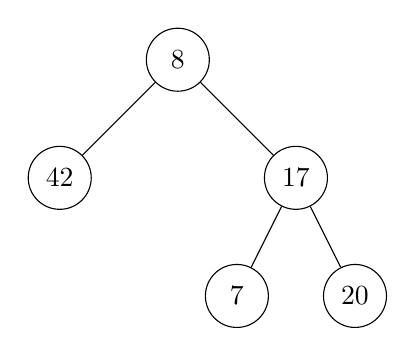
\begin{tikzpicture}[level distance=1.5cm,
  level 1/.style={sibling distance=3cm},
  level 2/.style={sibling distance=1.5cm},
  every node/.style={circle, draw, minimum size=0.8cm}]
  \node {8}
    child {node {42}}
    child {node {17}
      child {node {7}}
      child {node {20}}
    };
\end{tikzpicture}
\end{center}

Các nút được biểu diễn bằng hình tròn. Các nút của cây có thể chứa bất kỳ loại dữ liệu nào, nhưng trong ví dụ này mỗi nút chứa một số nguyên. Nút chứa $8$ là gốc của cây, với $42$ và $17$ là các con của nó. Cả $42$ và $17$ đều là gốc của các cây con. Ví dụ, cây con có gốc tại $17$ có ba nút: $17$ là gốc với các con là $7$ và $20$. Các nút không có con được gọi là \textbf{nút lá}. Trong cây ví dụ của chúng ta, các nút lá là $42$, $7$ và $20$.

Chúng ta sẽ hình thức hóa cấu trúc này---cây---khi chúng ta học về tập hợp và quan hệ trong chương tiếp theo, nhưng hiện tại chúng ta sẽ bằng lòng với định nghĩa phi hình thức sau:

\begin{definition}[Nút cây (phi hình thức)]
Một nút trong cây có a) một giá trị, b) một danh sách các nút.
\end{definition}

Có nhiều tên khác được sử dụng trong mô tả cây, và một số có thể khác một chút giữa các sách giáo khoa. Trong sách này, chúng ta sử dụng tập thuật ngữ sau. Lưu ý cách một số trong đó được định nghĩa đệ quy!

\begin{description}
\item[Nút cha của $x$] Nút mà trong danh sách các nút con có $x$ xuất hiện.
\item[Nút anh em của $x$] Các nút khác trong danh sách các con của nút cha của $x$.
\item[Hậu duệ của $x$] $x$ và các hậu duệ của các con của $x$.
\item[Tổ tiên của $x$] $x$ và các tổ tiên của nút cha của $x$.
\item[Lá] Nút không có con.
\item[Gốc] Nút không có nút cha.
\item[Cây nhị phân] Cây mà mỗi nút có tối đa $2$ con.
\item[Chiều cao] Số lượng đỉnh lớn nhất trên đường đi từ lá đến gốc, không tính lá.
\end{description}

Sử dụng thuật ngữ này, chúng ta có thể nói rằng cây ví dụ ở trên có chiều cao $2$, chứa $3$ lá, và là cây nhị phân. Hơn nữa, các tổ tiên của $20$ là $20$ chính nó, $17$ và $8$.

\subsection{Một ứng dụng của cây}

Cây phổ biến trong khoa học máy tính vì chúng có thể được sử dụng cho nhiều ứng dụng khác nhau, từ sắp xếp, đến quản lý bộ nhớ và theo dõi các thành viên gia đình (mặc dù trường hợp sau không hẳn là cây: bạn thấy tại sao không?). Trong môn \emph{Algorithms \& Data Structures} bạn cũng sẽ gặp nhiều ứng dụng này. Cây là loại đặc biệt của cấu trúc dữ liệu liên kết tổng quát hơn, đồ thị, cũng rất hữu ích trong khoa học máy tính. Chúng ta sẽ xem xét đồ thị trong chương tiếp theo.

Hiện tại chúng ta chỉ xem xét một ví dụ, sử dụng cây để biểu diễn các công thức toán học. Xem xét ví dụ biểu thức: $(8 + 3) * (10/5)$. Chúng ta có thể biểu diễn nó bằng cây, trong đó mỗi toán tử là gốc của một cây con, và các lá của cây là các số khác nhau:

\begin{center}
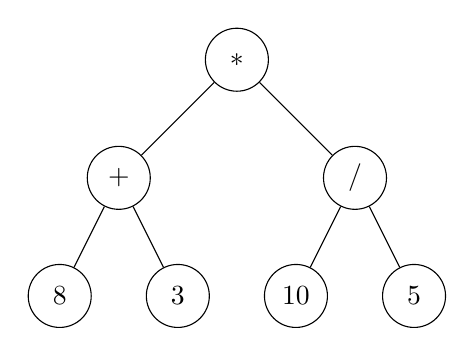
\begin{tikzpicture}[level distance=1.5cm,
  level 1/.style={sibling distance=3cm},
  level 2/.style={sibling distance=1.5cm},
  every node/.style={circle, draw, minimum size=0.8cm}]
  \node {$*$}
    child {node {$+$}
      child {node {$8$}}
      child {node {$3$}}
    }
    child {node {$/$}
      child {node {$10$}}
      child {node {$5$}}
    };
\end{tikzpicture}
\end{center}

Lưu ý cây này có các loại ``dữ liệu'' khác nhau trong các nút: một số là số và một số là toán tử.

Bạn sẽ thấy rằng với mỗi cây có đúng một biểu thức khớp với nó! Ví dụ, cây sau biểu diễn phát biểu: $\dfrac{x + 8}{(x+1)(y-1)} - 2$.

Nếu bạn đã có kinh nghiệm lập trình, có lẽ bạn đã có thể thấy cách này có thể là cách hữu ích để biểu diễn biểu thức toán học. Bây giờ chúng ta có thể viết thuật toán đệ quy đầu tiên tính giá trị của các con, và sau đó áp dụng toán tử tại gốc của cây con. Đơn giản là:
\begin{enumerate}
\item Nếu nút này là số, trả về số đó.
\item Ngược lại tính giá trị mỗi con.
\item Kết hợp các giá trị bằng toán tử trong nút này.
\end{enumerate}

Trong các bài tập bạn cũng sẽ thực hành chuyển các phát biểu logic mệnh đề và logic vị từ thành cây.

\subsection{Cây nhị phân trong Java}

Để có ví dụ về định nghĩa đệ quy và chứng minh quy nạp, chúng ta sẽ xem cấu trúc dữ liệu gọi là \textbf{cây nhị phân}. Như bạn có thể đoán từ tên gọi, và như chúng ta đã chỉ ra trước đó, cây nhị phân là một loại cây.

\begin{warningbox}
Nếu bạn chưa biết về đối tượng và con trỏ, bạn sẽ không thể theo dõi phần còn lại của mục này. Đã đến lúc đọc về nó trên internet?
\end{warningbox}

Giống như mọi cây, cây nhị phân gồm các nút liên kết với nhau theo cấu trúc giống cây. Cây nhị phân có thể rỗng, hoặc nó có thể gồm một nút (gốc của cây) và hai cây nhị phân nhỏ hơn (gọi là \textbf{cây con trái} và \textbf{cây con phải} của cây). Bạn đã có thể thấy cấu trúc đệ quy: cây có thể chứa các cây nhỏ hơn. Lưu ý rằng định nghĩa đệ quy này ngay lập tức giới hạn mỗi nút có tối đa hai con.

Trong ngôn ngữ lập trình Java, các nút của cây có thể được biểu diễn bởi các đối tượng thuộc lớp này:
\begin{lstlisting}[language=Java]
class BinaryTreeNode {
    int item;               // Gia tri so nguyen luu trong nut.
    BinaryTreeNode left;    // Con tro den cay con trai.
    BinaryTreeNode right;   // Con tro den cay con phai.
}
\end{lstlisting}

Cây rỗng được biểu diễn bằng con trỏ có giá trị đặc biệt \texttt{null}. Nếu \texttt{root} là con trỏ đến nút gốc của cây, thì \texttt{root.left} là con trỏ đến cây con trái và \texttt{root.right} là con trỏ đến cây con phải. Tất nhiên, cả \texttt{root.left} và \texttt{root.right} có thể là \texttt{null} nếu cây con tương ứng rỗng. Tương tự, \texttt{root.item} là tên cho số nguyên trong nút gốc.

Giả sử chúng ta muốn một hàm tìm tổng tất cả các số nguyên trong tất cả các nút của cây nhị phân. Chúng ta có thể làm điều này với hàm đệ quy đơn giản. Trường hợp cơ sở của đệ quy là cây rỗng. Vì không có số nguyên nào trong cây rỗng, tổng các số nguyên trong cây rỗng là không. Cho cây không rỗng, chúng ta có thể sử dụng đệ quy để tìm tổng các số nguyên trong cây con trái và phải, và sau đó cộng các tổng đó với số nguyên trong nút gốc. Trong Java, điều này có thể biểu diễn như sau:

\begin{lstlisting}[language=Java]
int TreeSum( BinaryTreeNode root ) {
    // Tim tong tat ca cac so nguyen trong
    // cay co goc da cho.
    int answer;
    if (root == null) {  // Cay rong.
        answer = 0;
    } else {
        answer = TreeSum(root.left);
        answer += TreeSum(root.right);
        answer += root.item;
    }
    return answer;
}
\end{lstlisting}

Chúng ta có thể sử dụng dạng thứ hai của nguyên lý quy nạp toán học để chứng minh hàm này đúng.

\begin{theorem}
Hàm \texttt{TreeSum}, định nghĩa ở trên, tính đúng tổng tất cả các số nguyên trong cây nhị phân.
\end{theorem}

\begin{proof}
Chúng ta sử dụng quy nạp theo số nút trong cây. Cho $P(n)$ là phát biểu ``\texttt{TreeSum} tính đúng tổng các nút trong bất kỳ cây nhị phân nào chứa đúng $n$ nút''. Chúng ta chứng minh $P(n)$ đúng cho mọi số tự nhiên $n$.

Xét trường hợp $n = 0$. Cây có không nút là rỗng, và cây rỗng được biểu diễn bằng con trỏ \texttt{null}. Trong trường hợp này, câu lệnh \texttt{if} trong định nghĩa \texttt{TreeSum} gán giá trị $0$ cho \texttt{answer}, và đây là tổng đúng cho cây rỗng. Vậy $P(0)$ đúng.

Cho $k$ là số tự nhiên tùy ý, với $k > 0$. Giả sử chúng ta đã biết $P(x)$ cho mỗi số tự nhiên $x$ với $0 \leq x < k$. Tức là, \texttt{TreeSum} tính đúng tổng tất cả các số nguyên trong bất kỳ cây nào có ít hơn $k$ nút. Chúng ta phải chứng minh $P(k)$ theo sau, tức là \texttt{TreeSum} hoạt động đúng cho cây có $k$ nút. Giả sử \texttt{root} là con trỏ đến nút gốc của cây có tổng cộng $k$ nút. Vì nút gốc chiếm một nút, còn lại tổng cộng $k - 1$ nút cho cây con trái và phải, nên mỗi cây con phải chứa ít hơn $k$ nút. Theo giả thiết quy nạp, chúng ta biết \texttt{TreeSum(root.left)} tính đúng tổng tất cả các số nguyên trong cây con trái, và \texttt{TreeSum(root.right)} tính đúng tổng tất cả các số nguyên trong cây con phải. Tổng tất cả các số nguyên trong cây là \texttt{root.item} cộng các tổng của số nguyên trong các cây con, và đây là giá trị được tính bởi \texttt{TreeSum}. Vậy \texttt{TreeSum} hoạt động đúng cho cây có $k$ nút. Điều này hoàn thành quy nạp.
\end{proof}

Lưu ý cấu trúc của chứng minh quy nạp theo sát cấu trúc của hàm đệ quy đến mức nào. Đặc biệt, nguyên lý quy nạp mạnh rất tự nhiên ở đây, vì kích thước của cây con có thể là bất kỳ giá trị nào đến nhỏ hơn kích thước cây hoàn chỉnh một đơn vị. Sẽ rất khó để sử dụng nguyên lý quy nạp thứ nhất trong chứng minh về cây nhị phân.

\subsection*{Bài tập}
\begin{exercise}
Vẽ cây nhị phân sao cho gốc có tổng cộng $8$ hậu duệ, và có nút có đúng $4$ tổ tiên.
\end{exercise}

\begin{exercise}
Giá trị của biểu thức được biểu diễn bởi cây sau là bao nhiêu?

\begin{center}
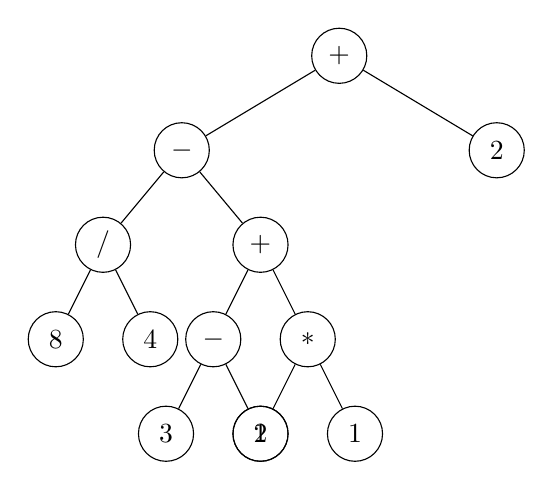
\begin{tikzpicture}[level distance=1.2cm,
  level 1/.style={sibling distance=4cm},
  level 2/.style={sibling distance=2cm},
  level 3/.style={sibling distance=1.2cm},
  every node/.style={circle, draw, minimum size=0.7cm, inner sep=1pt}]
  \node {$+$}
    child {node {$-$}
      child {node {$/$}
        child {node {$8$}}
        child {node {$4$}}
      }
      child {node {$+$}
        child {node {$-$}
          child {node {$3$}}
          child {node {$1$}}
        }
        child {node {$*$}
          child {node {$2$}}
          child {node {$1$}}
        }
      }
    }
    child {node {$2$}};
\end{tikzpicture}
\end{center}
\end{exercise}

\begin{exercise}
Vẽ cây cho phát biểu logic mệnh đề: $(p \wedge q) \to \neg(r \leftrightarrow z)$.
\end{exercise}

\begin{exercise}
Vẽ cây cho phát biểu logic vị từ: $\forall x(P(x) \to (Q(x) \vee \exists y(R(x, y))))$.
\end{exercise}

\begin{exercise}
Nút lá trong cây nhị phân là nút mà cả cây con trái và cây con phải đều rỗng. Chứng minh rằng hàm đệ quy sau đếm đúng số lá trong cây nhị phân:
\begin{lstlisting}[language=Java]
int LeafCount(BinaryTreeNode root) {
    // Dem so nut la trong
    // cay co goc da chi dinh.
    int count;
    if (root == null) {
        count = 0;
    } else if (root.left == null && root.right == null) {
        count = 1;
    } else {
        count = LeafCount(root.left);
        count += LeafCount(root.right);
    }
    return count;
}
\end{lstlisting}
\end{exercise}

\begin{exercise}
\textbf{Cây tìm kiếm nhị phân} thỏa mãn tính chất sau: Nếu \texttt{node} là con trỏ đến bất kỳ nút nào trong cây, thì tất cả các số nguyên trong cây con trái của \texttt{node} nhỏ hơn \texttt{node.item} và tất cả các số nguyên trong cây con phải của \texttt{node} lớn hơn hoặc bằng \texttt{node.item}. Chứng minh rằng chương trình con đệ quy sau in tất cả các số nguyên trong cây tìm kiếm nhị phân theo thứ tự không giảm:
\begin{lstlisting}[language=Java]
void SortPrint(BinaryTreeNode root) {
    // Gia su root la con tro den
    // nut goc cua cay tim kiem nhi phan. Chuong trinh
    // con nay in cac so nguyen trong
    // cay theo thu tu khong giam.
    if (root == null) {
        // Khong co gi de in.
    }
    else {
        SortPrint(root.left);
        System.out.println(root.item);
        SortPrint(root.right);
    }
}
\end{lstlisting}
\end{exercise}

\begin{exercise}
Mở rộng Định lý 3.14 cho cây không phải nhị phân.
\end{exercise}

%%%%%%%%%%%%%%%%%%%%%%%%%%%%%%%%%%%%%%%%%%%%%%%%%%%%%
\section{Bất biến}
%%%%%%%%%%%%%%%%%%%%%%%%%%%%%%%%%%%%%%%%%%%%%%%%%%%%%

Đệ quy liên quan chặt chẽ với lặp. Thực tế, một vòng lặp \texttt{while} có thể được viết dưới dạng chương trình con đệ quy (và đây là cách ngôn ngữ lập trình Prolog đạt được ``lặp'': xem trang 86). Trong khoa học máy tính, chúng ta muốn chứng minh tính đúng đắn và các tính chất khác về thuật toán. Các chứng minh về thuật toán có thể khó hơn các chứng minh về tính chất đơn giản của số nguyên mà chúng ta thường dùng làm ví dụ trong sách này.

Một công cụ giúp chúng ta chứng minh các tính chất về thuật toán là \textbf{bất biến}. Ví dụ, \textbf{bất biến vòng lặp} là tính chất $P$ của vòng lặp sao cho:
\begin{enumerate}
\item $P$ đúng trước khi vòng lặp được thực hiện, và
\item $P$ vẫn đúng sau mỗi lần thực hiện thân vòng lặp (nhưng không nhất thiết trong giữa các bước bên trong thân).
\end{enumerate}

Vậy để chứng minh thuật toán $A$ có tính chất $Q$ (hậu điều kiện), chúng ta có thể tìm bất biến $P$ của $A$ sao cho $Q$ theo sau từ $P$, cùng với thực tế rằng $A$ đã kết thúc. Thực tế cuối cùng rằng $A$ đã kết thúc nghĩa là điều kiện vòng lặp (bộ canh vòng lặp) đã trở thành sai.

Chi tiết hơn, chúng ta cần tìm bất biến và chứng minh bốn điều về nó:
\begin{enumerate}
\item \textbf{Khởi tạo hay tính chất cơ sở.} Bất biến đúng trước lần lặp đầu tiên.
\item \textbf{Duy trì hay tính chất quy nạp.} Nếu bất biến đúng trước một lần lặp, thì nó cũng đúng trước lần lặp tiếp theo.
\item \textbf{Kết thúc và tính sai của bộ canh.} Sau hữu hạn lần lặp, bộ canh trở thành sai và vòng lặp kết thúc.
\item \textbf{Tính đúng của hậu điều kiện.} Bất biến cùng với phủ định của bộ canh suy ra hậu điều kiện đúng, trong trường hợp đó chương trình đúng.
\end{enumerate}

Ví dụ, xét vòng lặp đơn giản:
\begin{lstlisting}
while (x < 10)
    x = x+1;
\end{lstlisting}

Vòng lặp này đạt được gì? Bất biến nào giúp chúng ta chứng minh vòng lặp đạt được điều đó đúng? Bất biến là $x \leq 10$---hãy kiểm tra rằng nó thỏa mãn bốn tính chất trên!

Mặc dù bất biến có thể hữu ích, tìm bất biến phù hợp có thể khó.

Cho ví dụ phức tạp hơn, xét đoạn mã sau. Lưu ý rằng bạn nên gọi đoạn mã này với số nguyên $n \geq 0$ và $a > 0$.
\begin{lstlisting}
r = 0
b = n
while (b >= a)
    b -= a
    r += 1
\end{lstlisting}

Hãy thử thuyết phục bản thân rằng đoạn mã này tính: $\lfloor n/a \rfloor$. Không tin chúng tôi? Chúng tôi sẽ chứng minh cho bạn:

\begin{proof}
Bất biến: $r \cdot a + b = n$.

\begin{enumerate}
\item \textbf{Khởi tạo hay tính chất cơ sở.} Trước khi vòng lặp chạy, $b = n$ và $r = 0$. Do đó $r \cdot a + b = b = n$.

\item \textbf{Duy trì hay tính chất quy nạp.} Giả sử bất biến đúng trước lần lặp $k$, tức là: $r_{\text{cũ}} \cdot a + b_{\text{cũ}} = n$.

Bây giờ ta chứng minh nó đúng sau lần lặp $k$, tức là: $r_{\text{mới}} \cdot a + b_{\text{mới}} = n$.

Từ dòng 4 ta suy ra: $b_{\text{mới}} = b_{\text{cũ}} - a$ và $r_{\text{mới}} = r_{\text{cũ}} + 1$. Do đó
\[r_{\text{mới}} \cdot a + b_{\text{mới}} = (r_{\text{cũ}} + 1) \cdot a + b_{\text{cũ}} - a = r_{\text{cũ}} \cdot a + a + b_{\text{cũ}} - a = r_{\text{cũ}} \cdot a + b_{\text{cũ}} \stackrel{\text{GT}}{=} n.\]

\item \textbf{Kết thúc và tính sai của bộ canh.} Mỗi lần lặp $b$ giảm đi $a$. Vì $a > 0$, điều này nghĩa là cuối cùng $b < a$ sẽ đúng.

\item \textbf{Tính đúng của hậu điều kiện.} Vì $0 \leq b < a$ và $r \cdot a + b = n$, ta biết rằng: $r \cdot a \leq n$ và $n = r \cdot a + b < r \cdot a + a < (r + 1) \cdot a$. Vậy ta được: $r \leq n/a$ và $n/a < r + 1$, do đó $n/a - 1 < r \leq n/a$. Vì $r$ là số nguyên, điều này nghĩa là: $r = \lfloor n/a \rfloor$.
\end{enumerate}
\end{proof}

\begin{infobox}
Có một dạng logic, \textbf{logic Floyd--Hoare}, trong đó chúng ta có thể biểu diễn bất biến và có thể chứng minh hình thức tính đúng đắn (một phần) của chương trình. Đọc về nó trên Wikipedia: \texttt{en.wikipedia.org/wiki/Loop\_invariant}.
\end{infobox}
